\documentclass[aspectratio=169,t]{beamer}

\definecolor{myaccent}{HTML}{356AE6}
\usetheme[
  accent=myaccent,
  progressbar=none,
  sectionpage=simple,
  subsectionpage=none,
  numbering=fraction,
  titleformat=regular,
  block=fill
]{cookie}

% Redefine the theme's paper color to pure white. This drives the background on
% content, section, and title pages (all keyed to cookiePaper) instead of the
% theme's default cream (#FBFAF7).
\definecolor{cookiePaper}{HTML}{FFFFFF}

% Render equations in the classic serif math font (Latin Modern / Computer
% Modern) instead of the theme's sans-serif default. [onlymath] leaves the
% body text in Fira Sans and only affects math.
\usefonttheme[onlymath]{serif}

% Override Cookie's section divider so it also lists the section's subsections
% as sub-points. This keeps the theme file pristine; it copies the theme's
% section page and adds a \tableofcontents[currentsection] node (subsections
% only) below the title. \cookie@format / colors are the theme's own macros.
\makeatletter
\setbeamertemplate{subsection in toc}{%
  \leavevmode\leftskip=2em\rlap{\raise.05ex\hbox{\textbullet}}\hskip1em%
  \inserttocsubsection\par%
}
\renewcommand{\cookie@sectionpageframe}{%
  \begin{frame}[plain,noframenumbering,c]
    \begin{tikzpicture}[remember picture,overlay]
      \fill[cookieAccent]
        (current page.south west) rectangle ($(current page.north west)+(.012\paperwidth,0)$);
      \node[anchor=west,text=cookieAccent,font=\fontsize{46}{46}\selectfont\bfseries]
        at ($(current page.west)+(.07\paperwidth,.22\paperheight)$) {\insertsectionnumber};
      \node[anchor=west,text width=.80\paperwidth,align=left]
        at ($(current page.west)+(.07\paperwidth,.10\paperheight)$)
        {{\usebeamerfont{section title}\usebeamercolor[fg]{section title}\cookie@format{\insertsection}}};
      \node[anchor=north west,text width=.80\paperwidth,align=left]
        at ($(current page.west)+(.07\paperwidth,-.04\paperheight)$)
        {\begin{minipage}{.80\paperwidth}%
           \fontsize{14}{16}\selectfont\usebeamercolor[fg]{normal text}%
           \tableofcontents[currentsection,%
             sectionstyle=hide/hide,%
             subsectionstyle=show/show/hide]%
         \end{minipage}};
      \fill[cookieAccent] ($(current page.east)+(-.095\paperwidth,.24\paperheight)$) circle[radius=.014\paperheight];
      \fill[cookieAccent,opacity=.45] ($(current page.east)+(-.072\paperwidth,.18\paperheight)$) circle[radius=.008\paperheight];
    \end{tikzpicture}
  \end{frame}%
}
\makeatother

% Shared bibliography with the thesis: natbib + BibTeX (apj style), pointing at
% thesis/references.bib. build.sh puts thesis/ on BIBINPUTS/BSTINPUTS so the
% .bib and apj.bst are found without copying them here.
\usepackage[authoryear,round,sort]{natbib}
% apj/AAS convention puts no comma between author and year: "(Nita 2010)".
% \bibpunct args: open, close, separator between cites, style (a=author-year),
% separator between author and year, separator between multiple years.
\bibpunct{(}{)}{;}{a}{}{,}
\usepackage{booktabs}

\title{Radio Recombination Line Forecasts with CHORD}
\author[Duncan Cameron-Steinke]{
  Duncan Cameron-Steinke\\[1ex] 
  {\small Supervisor: Dr.~Alex Hill} \\[1ex] 
  {\small The University of British Columbia, Okanagan,\\ Irving K. Barber Faculty of Science}
}
\date{July 30, 2026}

\begin{document}
\maketitle

\makeagenda

\section{Motivation \& Background}

\subsection{Research Goal}
\begin{frame}{Motivation}{}
  \centering
  \par\medskip
  \par\medskip
  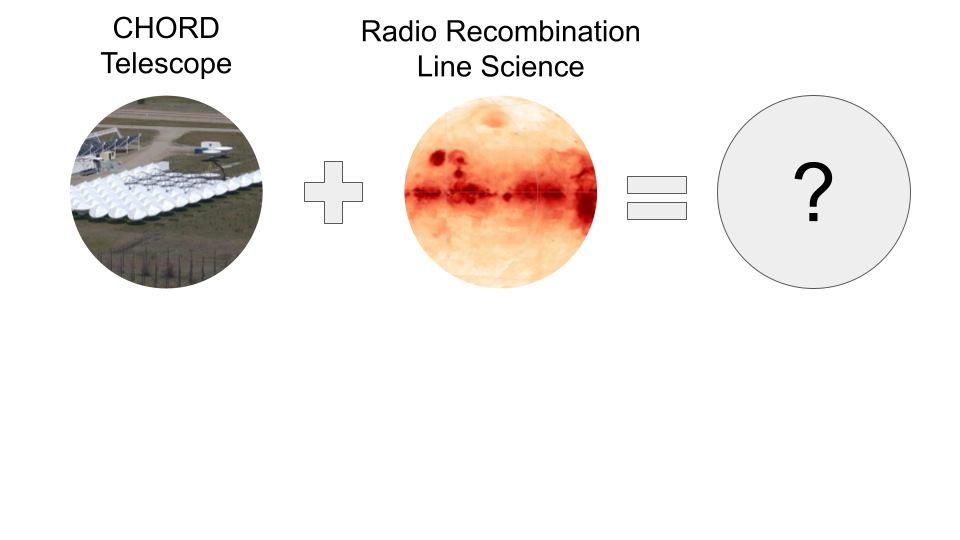
\includegraphics[width=0.9\linewidth,clip,trim=0 180pt 0 0]{plots/motivation_slide.png}
  \begin{itemize}
    \item Will CHORD detect Hydrogen Radio Recombination Lines?\\
    \par\medskip
    \item If so, what angular resolution and sensitivity can be achieved?
  \end{itemize}
\end{frame}

\subsection{Physics Background}
\begin{frame}{The Canadian Hydrogen Observatory and Radio-transient Detector (CHORD)}{}
  \begin{columns}[T]
    \begin{column}{0.5\linewidth}
      \begin{itemize}
        \item CHORD is a drift scan interferometer radio telescope:\\
        \begin{itemize}
          \item \textbf{Drift scan}: the telescope is fixed and the sky drifts overhead.
          \item \textbf{Interferometer}: 512 dishes work together to form a single sky image.
          \item \textbf{Radio telescope}: CHORD measures from $300-1500$ MHz.
        \end{itemize}
        \item CHORD Pathfinder will be operational in 2026, with the full CHORD array operational in 2028.
      \end{itemize}
    \end{column}
    \begin{column}{0.4\linewidth}
      \centering
      {\usebeamercolor[fg]{structure}CHORD under construction}
      \par\smallskip
      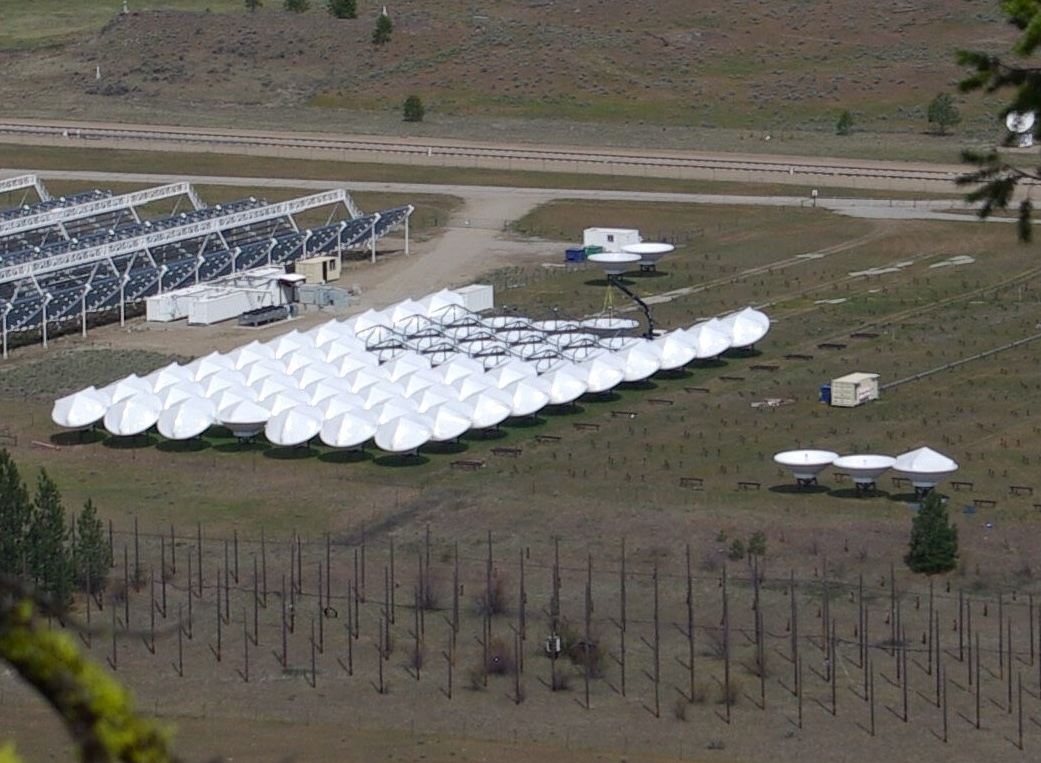
\includegraphics[width=0.8\linewidth]{plots/CHORD.jpeg}
      \par\medskip
      {\footnotesize CHORD is situated at the Dominion Radio Astrophysical Observatory (DRAO) \citep{SPIEpaper}}
    \end{column}
  \end{columns}
\end{frame}

\begin{frame}{Radio Recombination Lines}{}
  \begin{columns}[T]
    \begin{column}{0.5\linewidth}
      \begin{itemize}
        \item When an electron recombines with an ion, it emits a stream of photons.
        \item Each transition emits a photon of a different frequency.
        \item Radio recombination lines (RRLs) are photons in the radio range.
        % \item Line intensity is inversely proportional to frequency; RRLs are stronger at low frequency.
      \end{itemize}
    \end{column}
    \begin{column}{0.4\linewidth}
      \centering
      {\usebeamercolor[fg]{structure}Bohr atomic model}
      \par\smallskip
      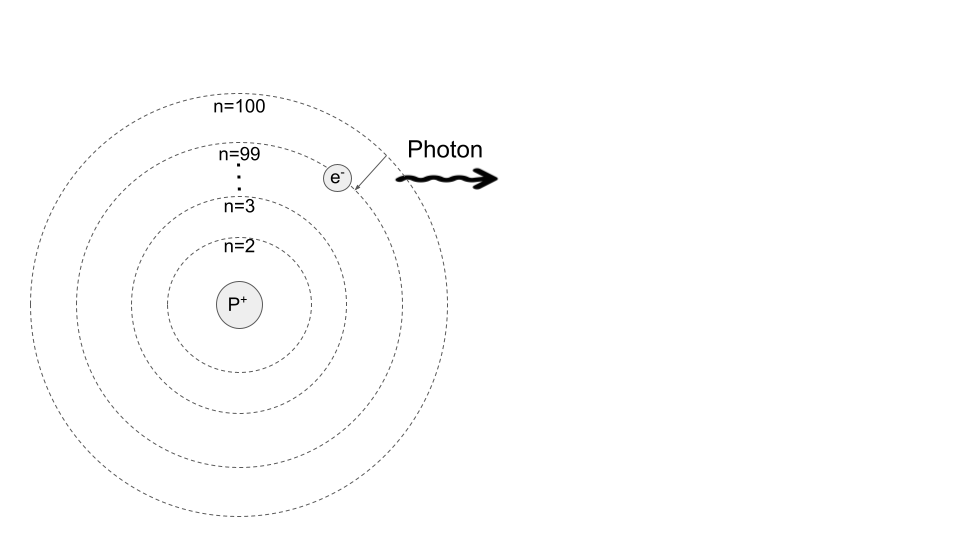
\includegraphics[width=0.8\linewidth, clip, trim=0 0 400pt 40pt]{plots/rrl_model.png}
      \par\medskip
      {\footnotesize Simplified Bohr model of the hydrogen atom showing RRL emission from $N=100 \to 99$.}
    \end{column}
  \end{columns}
\end{frame}

\begin{frame}{The Interstellar Medium (ISM)}{}
  \begin{columns}[T]
    \begin{column}{0.5\linewidth}
      Why measure RRLs?\\
      \begin{itemize}
        \item RRLs are produced in ionized regions of the interstellar medium (ISM). 
        \item Studying the ionized ISM teaches us about star formation and galactic evolution.
        \item RRLs travel further compared to optical emission, providing an extended view of the ISM.
      \end{itemize}
    \end{column}
    \begin{column}{0.5\linewidth}
      \centering
      {\usebeamercolor[fg]{structure}Wisconsin H$\alpha$ Mapper sky survey}
      \par\smallskip
      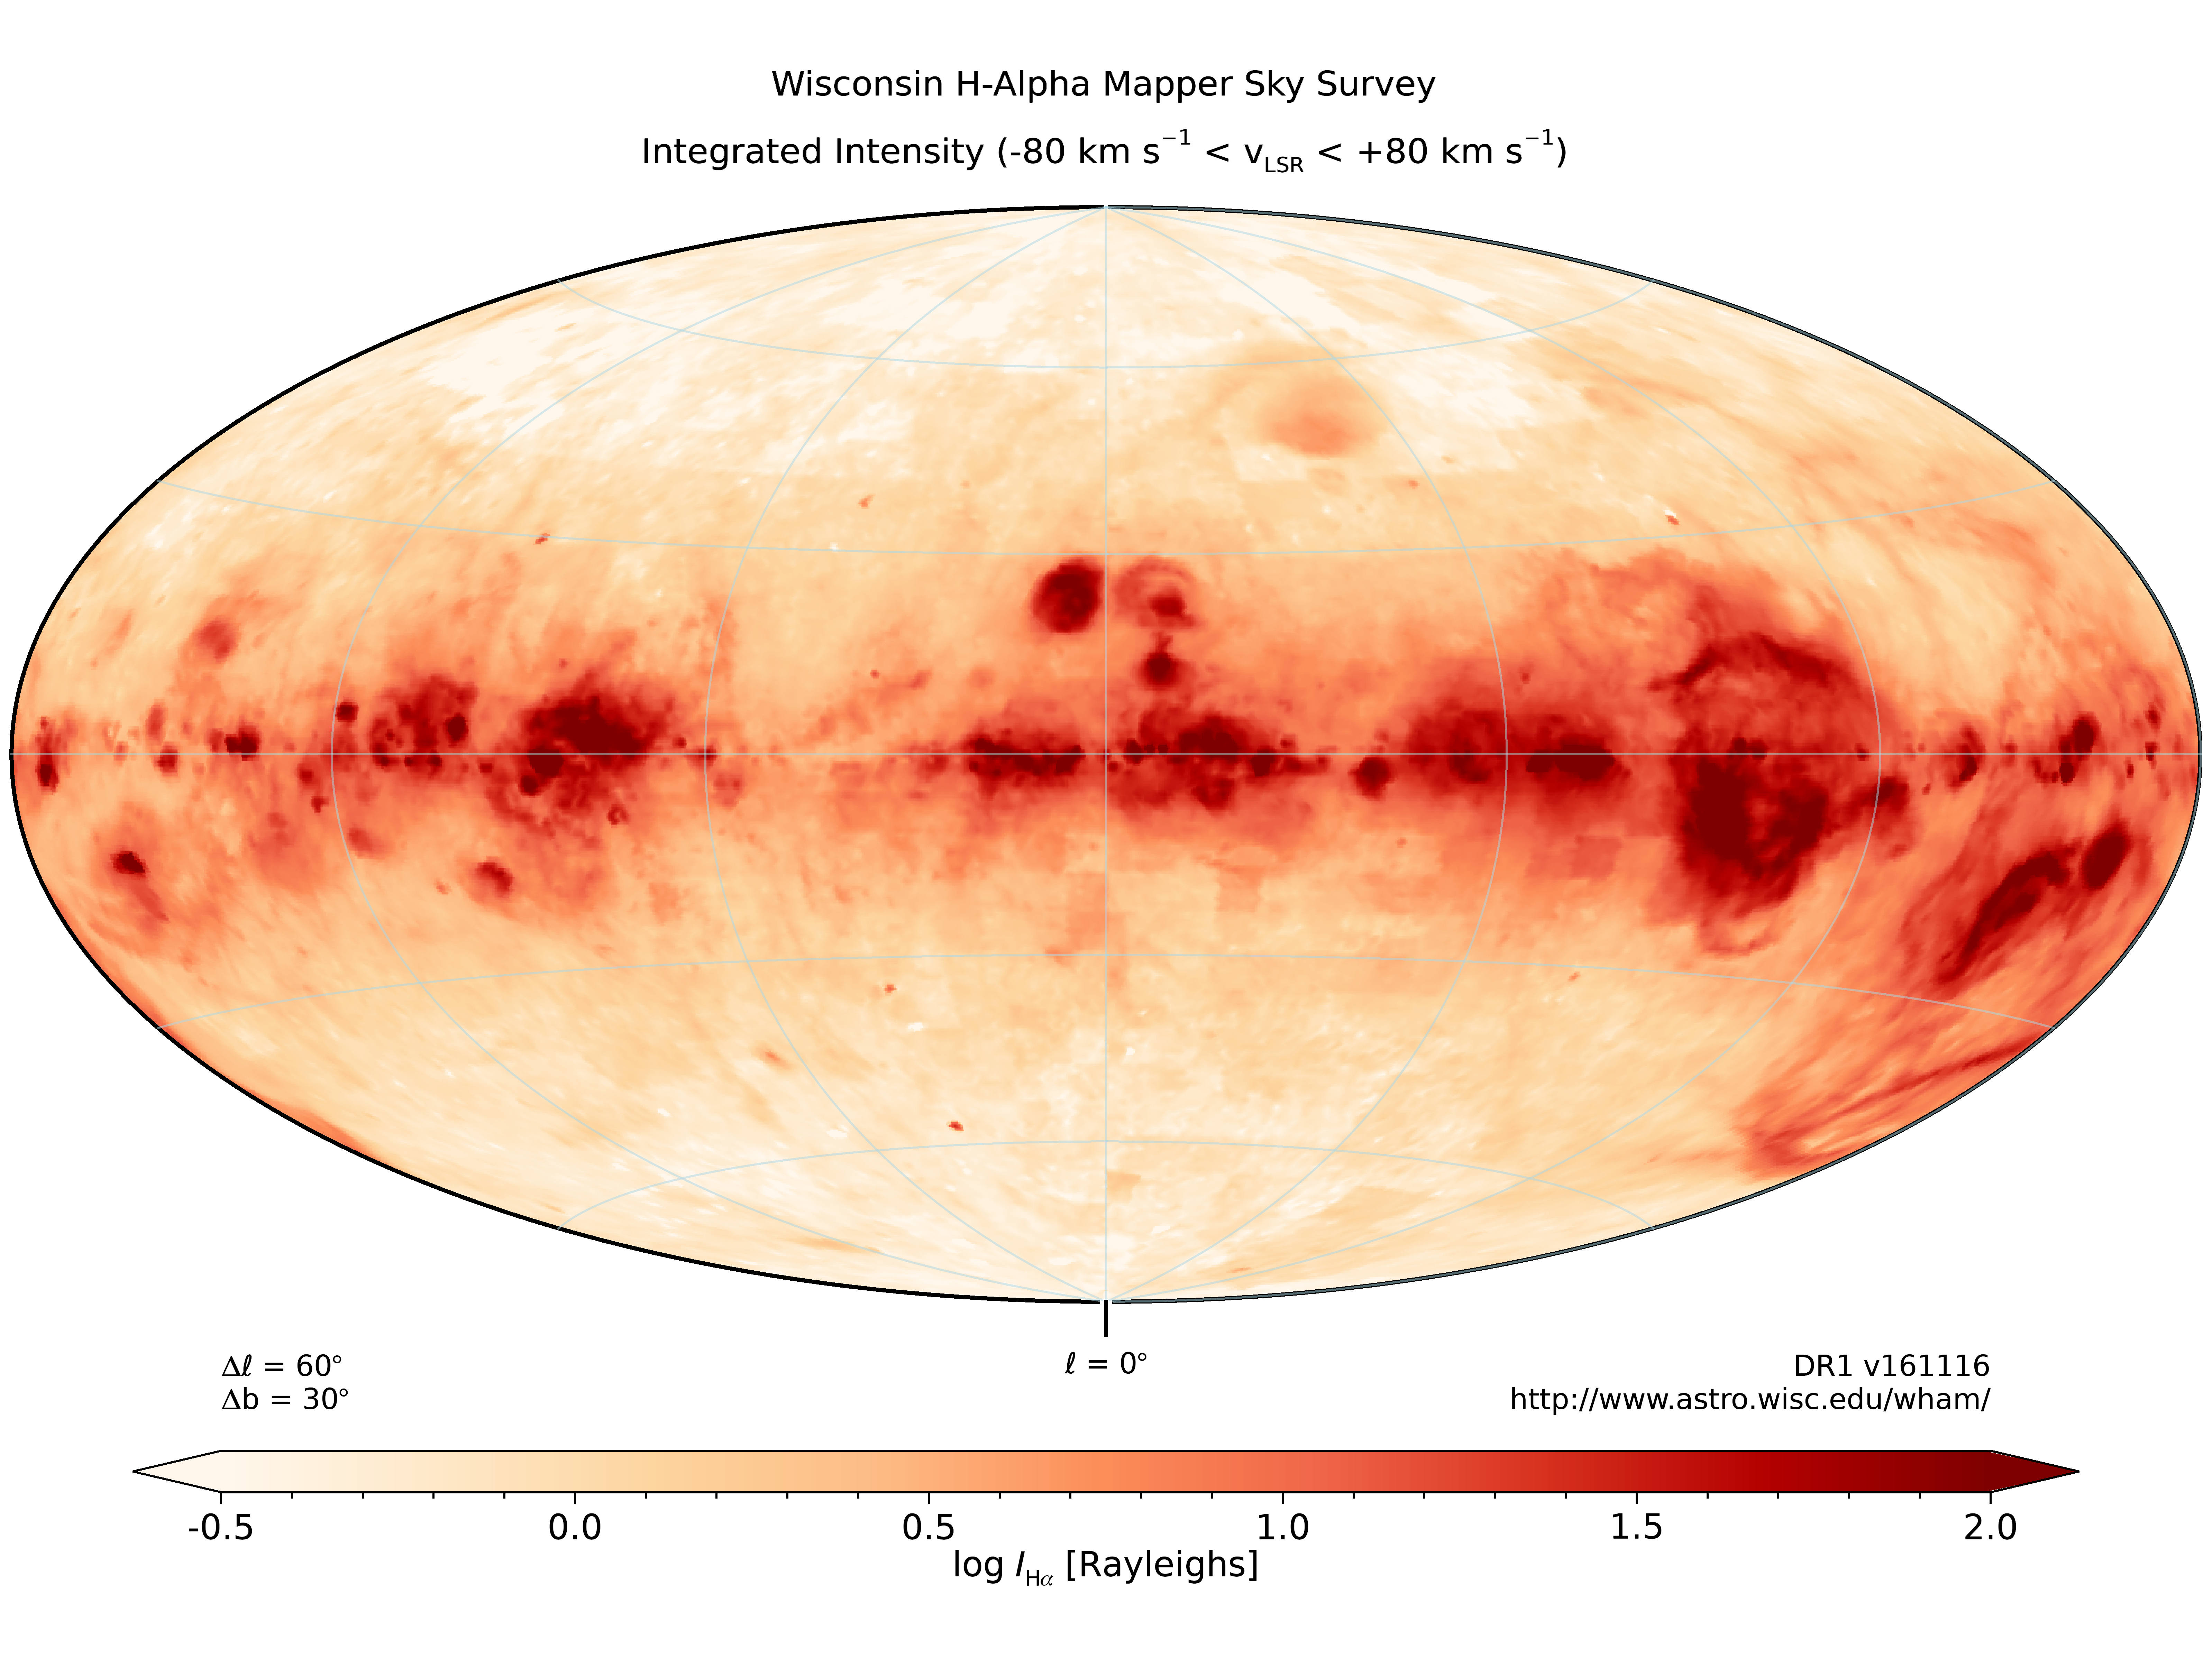
\includegraphics[width=0.8\linewidth,clip,trim=0 20pt 0 60pt]{plots/wham_image.png}
      \par\medskip
      {\footnotesize All-sky map of H$\alpha$ emission in the visible spectrum showing the ionized ISM \citep{haffnerEarlyResultsWisconsin2010}.}
    \end{column}
  \end{columns}
\end{frame}


\section[RFI]{Radio Frequency Interference}
\subsection{What is RFI}
\begin{frame}{Definition of RFI}{}
  \begin{columns}[T]
    \begin{column}{0.5\linewidth}
      \begin{itemize}
        \item Radio Frequency Interference (RFI) are unwanted human-made signals.
        \item Astronomical Signals are Gaussian distributed, while RFI is non-Gaussian.
      \end{itemize}
      \par\medskip
      To detect an RRL, we need to ensure there is no competing RFI.
    \end{column}
    \begin{column}{0.45\linewidth}
      \centering
      {\usebeamercolor[fg]{structure}Examples of RFI}
      \par\smallskip
      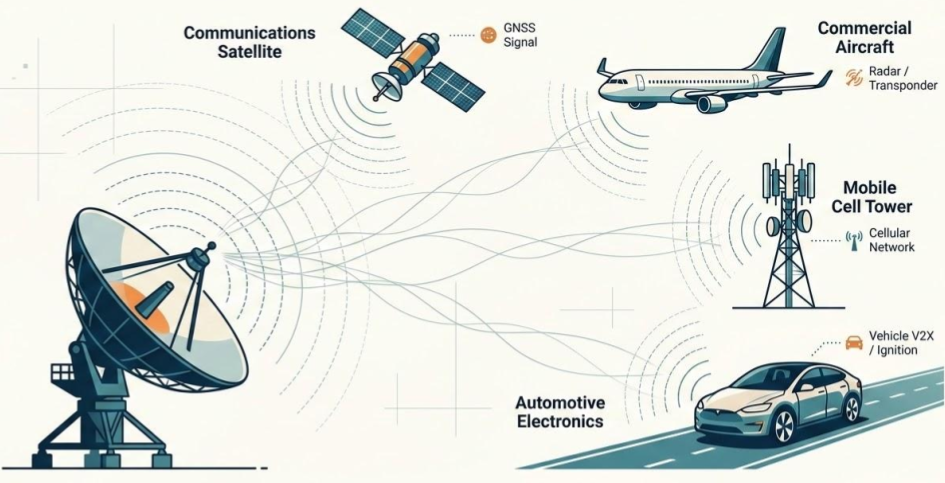
\includegraphics[width=1\linewidth]{plots/RFI_examples.png}
      \par\medskip
      {\footnotesize Sources of RFI can include satellites, aircraft, mobile phones, and cars. \citep{RFI_image}}
    \end{column}
  \end{columns}
\end{frame}

\subsection{How to detect RFI}
\begin{frame}{RFI-Monitor Data}{}
  \begin{columns}[T]
    \begin{column}{0.5\linewidth}
      Analysis of RFI-Monitor data statistics:
      \begin{enumerate}
        \item Complex voltages are measured and converted to power
        \[P = |V|^2 \sim \text{Exp}(2\sigma^2). \]
        \item Power is integrated into $0.75s$ windows over $N = 2500$ time samples
        \[P_N = \sum_{i=1}^{N} P_i \sim \text{Gamma}(N, 2\sigma^2).\]
      \end{enumerate}

      \footnotesize{RFI-monitor data provided by Nick Bruce, DRAO.}
    \end{column}
    \begin{column}{0.45\linewidth}
      \centering
      {\usebeamercolor[fg]{structure}DRAO RFI Monitor}
      \par\smallskip
      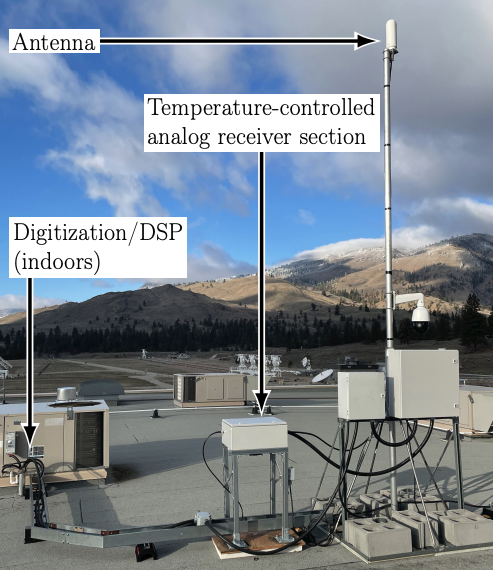
\includegraphics[width=0.6\linewidth]{plots/RFI_monitor.png}
      \par\medskip
      {\footnotesize The roof mounted DRAO RFI-Monitor which measures all incoming radio signals \citep{bruceWidebandRFIMonitor2026}.}
    \end{column}
  \end{columns}
\end{frame}

% \subsection{RFI Detection}
\begin{frame}{RFI Detection}{}
  \begin{columns}[T]
    \begin{column}{0.5\linewidth}
      I applied the generalized Spectral Kurtosis (SK) \citep{nitaGeneralizedSpectralKurtosis2010} estimator to detect RFI.
      \begin{itemize}
        \item I showed how to calibrate the SK estimator on RFI free data.
        \item I found that SK must be computed within RFI monitor calibration cycles.
        \item I showed that the SK estimator could accurately detect RFI.
      \end{itemize}
      
    \end{column}
    \begin{column}{0.5\linewidth}
      \centering
      {\usebeamercolor[fg]{structure}Power and SK on 600 MHz spectrum}
      \par\smallskip
      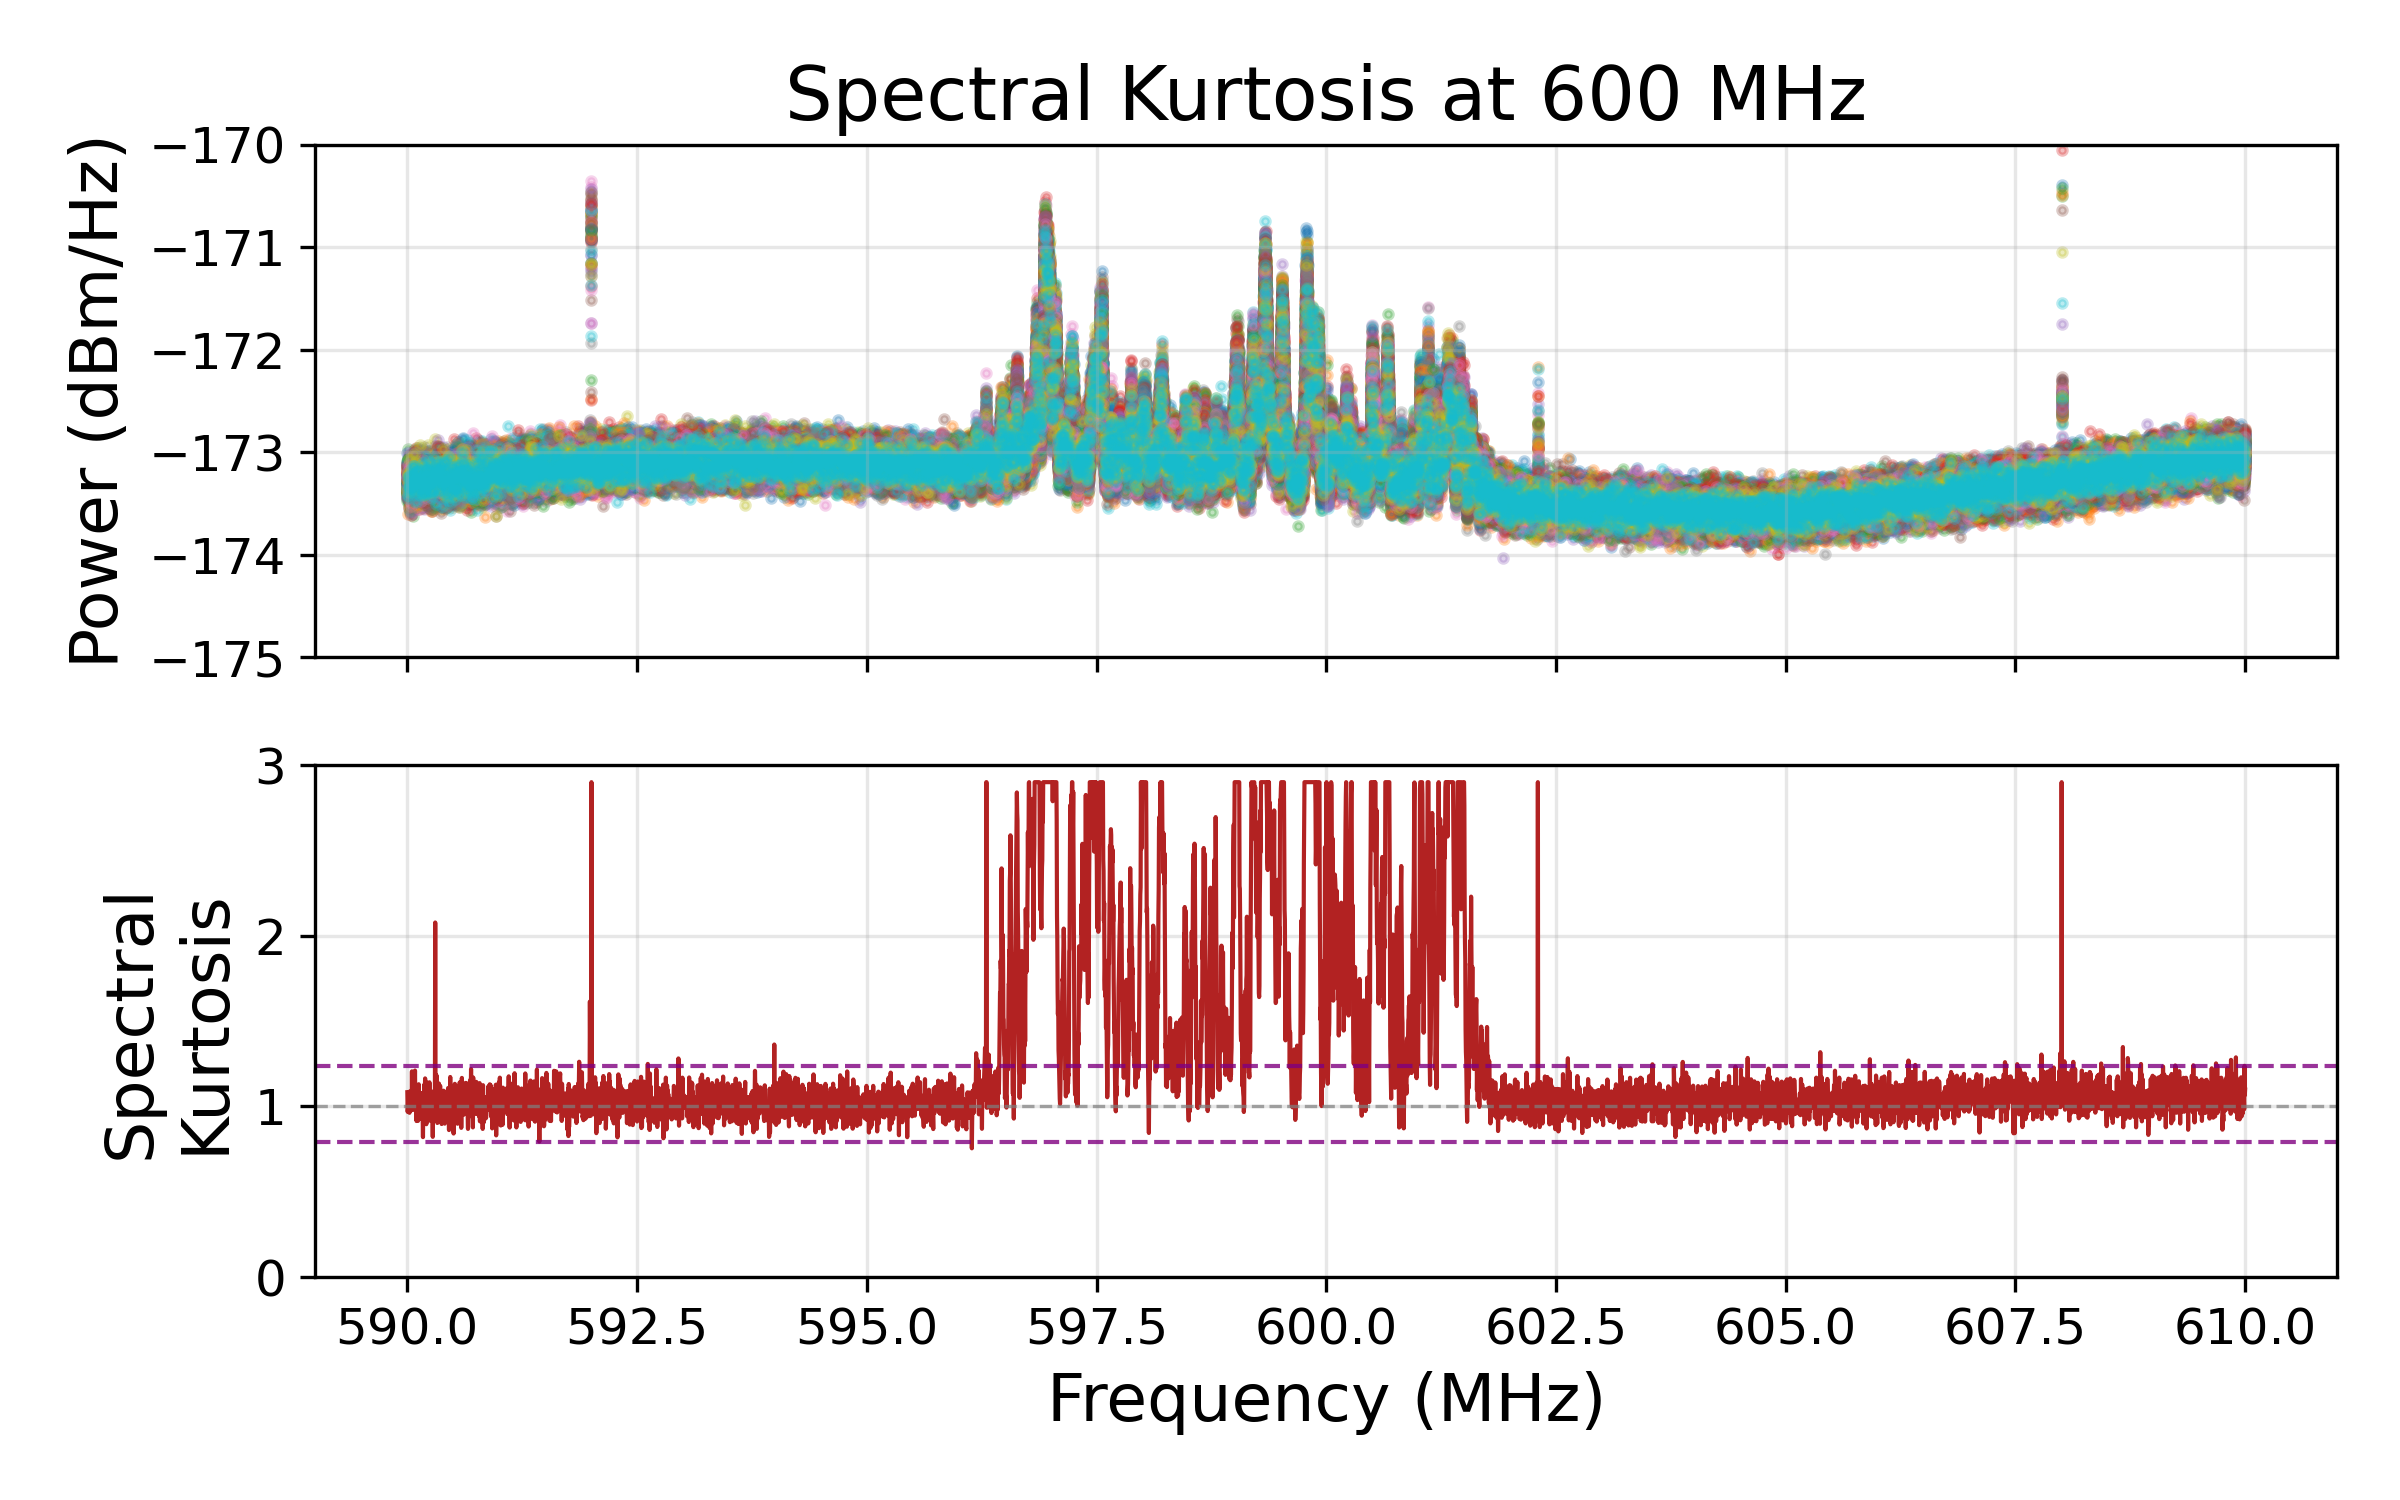
\includegraphics[width=1\linewidth, clip,trim=0 0 0 32pt]{../thesis/plots/rfi/600MHz_sample_SK.png}
      \par\medskip
      {\footnotesize Top plot shows RFI Monitor data. Bottom plot shows calibrated spectral kurtosis.}
    \end{column}
  \end{columns}
\end{frame}

\begin{frame}{Detection Thresholds}{}
  \begin{columns}[T]
    \begin{column}{0.5\linewidth}
      I obtained principled RFI detection thresholds and showed they conformed with observed RFI free data.
      \begin{itemize}
        \item Simulated the theoretical SK distribution (blue).
        \item Observed SK distribution (yellow).
        \item I selected 0.1\% and 99.9\% percentiles as RFI detection thresholds.
      \end{itemize}
    \end{column}
    \begin{column}{0.5\linewidth}
      \centering
      {\usebeamercolor[fg]{structure}SK distribution of RFI free data}
      \par\smallskip
      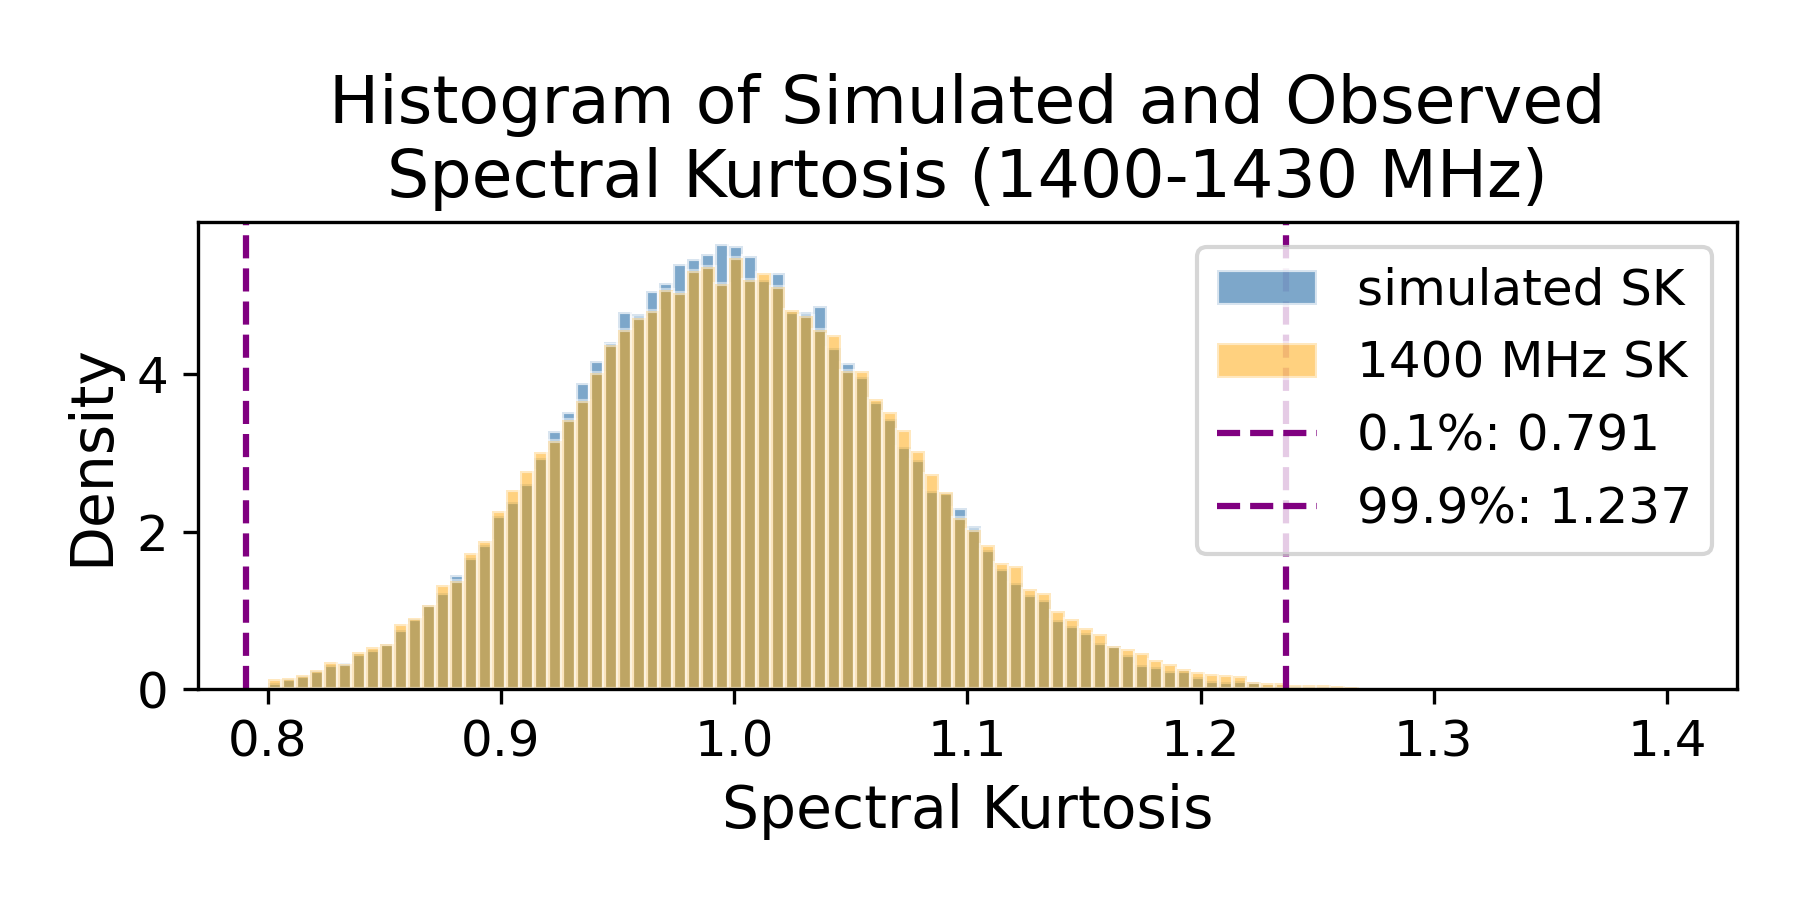
\includegraphics[width=1\linewidth, clip,trim=0 0 0 51pt]{../thesis/plots/rfi/spectral_kurtosis_all_time.png}
      \par\medskip
      {\footnotesize Theoretical SK distribution (blue) matches observed non-RFI SK distribution (yellow).}
    \end{column}
  \end{columns}
\end{frame}

\subsection{RFI impact on Radio Recombination Lines}
\begin{frame}{RFI across the full CHORD Spectrum}{}
  \centering
  {\usebeamercolor[fg]{structure}RFI across the full CHORD Spectrum}
  \par\smallskip
  \includegraphics[width=0.7\linewidth, clip,trim=0 10pt 0 33pt]{../thesis/plots/rfi/RFI_flagged_spectrum.png}
  \par\smallskip
  {\footnotesize RFI-monitor power colored by RFI flagging.}
  \par\medskip
  \begin{itemize}
    \item I found that 75.6\% of the CHORD band is RFI free.\\
    \item The GNSS band (1215-1300 MHz) shows less RFI then expected.\\
  \end{itemize}
\end{frame}

\begin{frame}{Clean Scores}{}
  \centering
  {\usebeamercolor[fg]{structure}Per line clean scores}
  \par\smallskip
  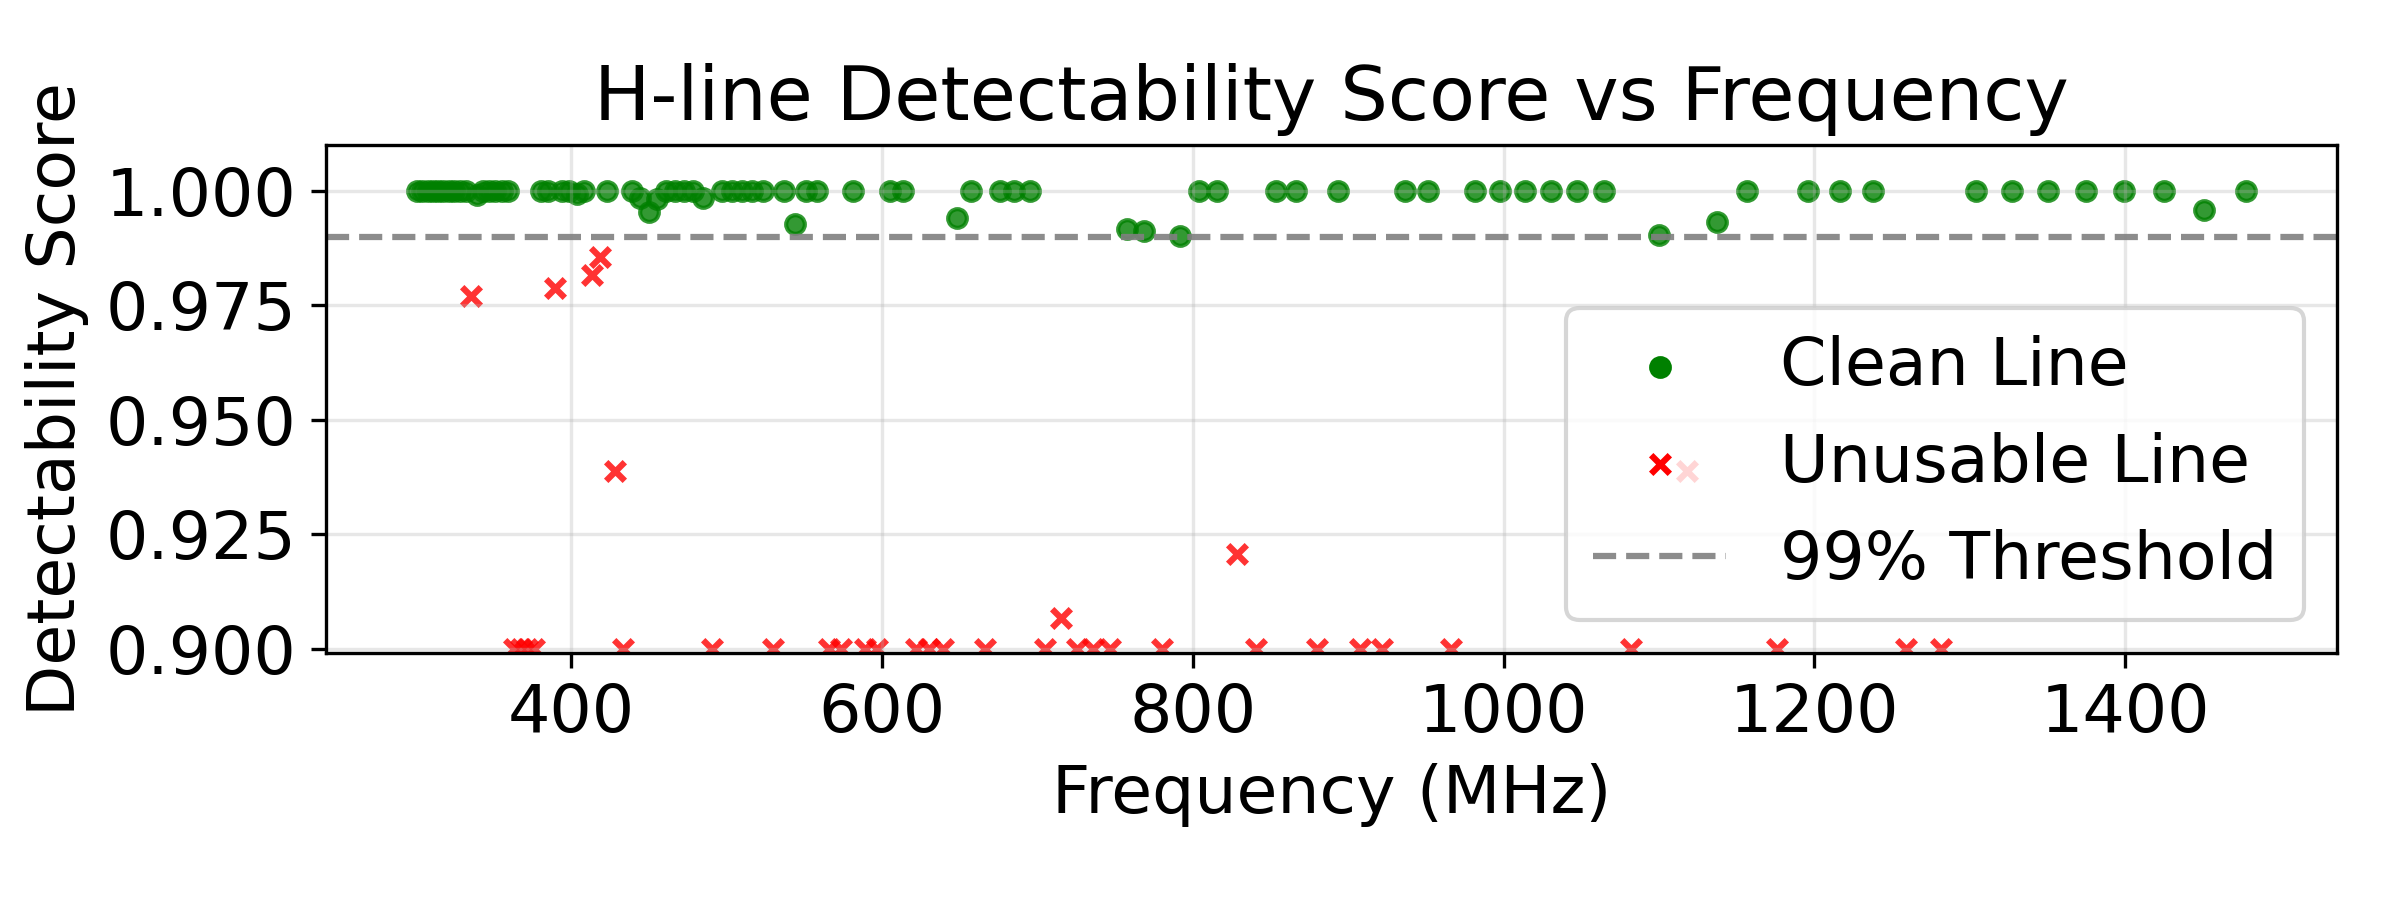
\includegraphics[width=0.7\linewidth, clip,trim=0 10pt 0 33pt]{../thesis/plots/rfi/h_line_clean_score.png}
  \par\smallskip
  {\footnotesize Gaussian weighted average around each RRL with a $100$ km s$^{-1}$ standard deviation.}
  \par\medskip
  \par\medskip
  \begin{itemize}
    \item I found that 79 of the 116 Hn$\alpha$ RRLs are RFI free.
  \end{itemize}
\end{frame}

\begin{frame}{RFI Analysis Limitations}{}
\begin{itemize}
    \item RFI-monitor sensitivity differs from CHORD.
    \par\medskip
    \item The RFI-monitor is angled towards the ground and horizon.
    \par\medskip
    \item The available data was limited to a single hour.
    \par\medskip
    \item The RFI environment might change in the future.
\end{itemize}
\end{frame}

\section{CHORD Sensitivity to RRLs}
\subsection{CHORD sensitivity maps}
\begin{frame}{Sensitivity Definitions}{Point Source Sensitivity}
  CHORD's point source sensitivity is computed as
  \[
  \sigma_{\mathrm{RMS}}\,[\mathrm{Jy/beam}] = \frac{2k\,(T_{\mathrm{ant}}+T_{\mathrm{sky}})}{A_e\sqrt{2\,\Delta\nu\,\tau_{\mathrm{eff}}\,N(N-1)}}
  \]
  where
  \begin{itemize}
    \item $k$ is Boltzmann's constant
    \item $T_{\mathrm{ant}}$ is the antenna temperature
    \item $T_{\mathrm{sky}}$ is the sky temperature
    \item $A_e$ is the effective area of a single dish
    \item $\Delta\nu$ is the bandwidth
    \item $\tau_{\mathrm{eff}}$ is the effective integration time
    \item $N$ is the number of dishes.
  \end{itemize}
  % where $k$ is Boltzmann's constant, $T_{\mathrm{ant}}$ is the antenna temperature, $T_{\mathrm{sky}}$ is the sky temperature, $A_e$ is the effective area of a single dish, $\Delta\nu$ is the bandwidth, $\tau_{\mathrm{eff}}$ is the effective integration time, and $N$ is the number of dishes.
\end{frame}

\begin{frame}{Sensitivity Definitions}{Brightness Temperature Sensitivity}
  RRLs are extended sources, so we need to convert from point-source sensitivity to brightness temperature sensitivity\\
  ~\\
  \[
  \sigma_T\,[\mathrm{K}] = \frac{\sigma_{\mathrm{RMS}}}{\Omega_s}\,
\frac{c^2}{2k\nu^2}
  \]
  where
  \begin{itemize}
    \item $\Omega_s$ is the solid angle of the synthesized beam
    \item $c$ is the speed of light
    \item $\nu$ is the observing frequency
  \end{itemize}
\end{frame}

\begin{frame}{Sensitivity Maps}{Intrinsic CHORD Brightness Temperature Sensitivity}
  \begin{columns}[T]
    \begin{column}{0.5\linewidth}
      Brightness temperature sensitivity if $T_{\mathrm{sky}}=0$\\
      \begin{itemize}
        \item Low Frequency has a larger primary beam.\\
        \item High declination has longer integration time.\\
      \end{itemize}
    \end{column}
    \begin{column}{0.5\linewidth}
      \centering
      {\usebeamercolor[fg]{structure}Intrinsic CHORD Sensitivity}
      \par\smallskip
      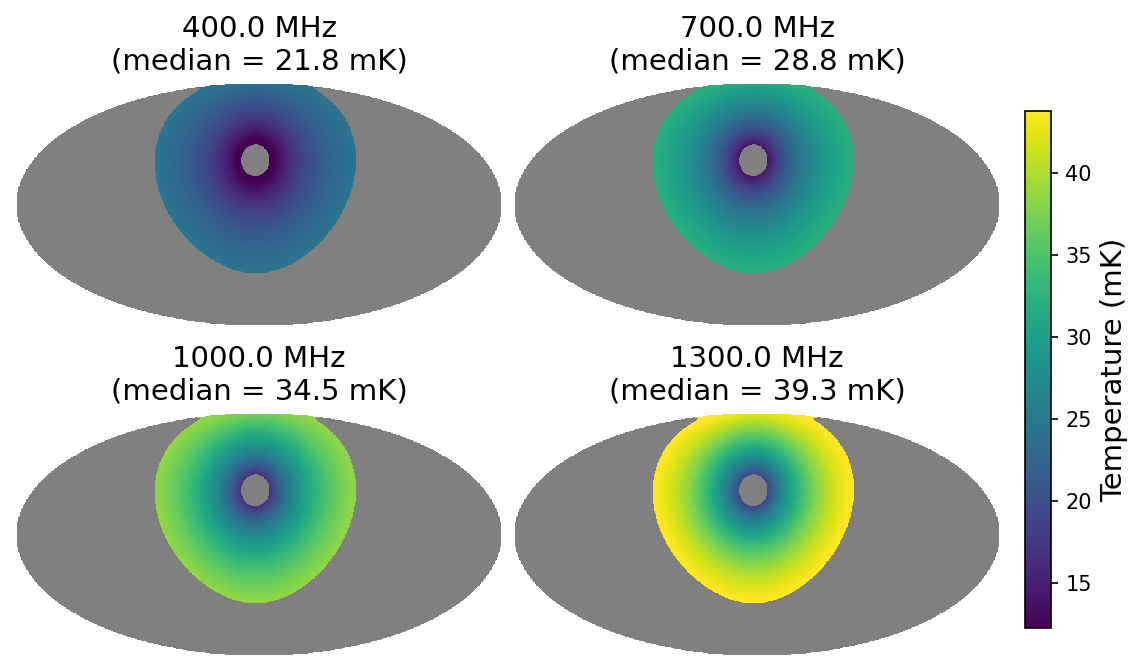
\includegraphics[width=1\linewidth]{../thesis/plots/sensitivity/system_only_noise.png}
      \par\medskip
      {\footnotesize Intrinsic CHORD brightness temperature sensitivity in galactic coordinates.}
    \end{column}
  \end{columns}
\end{frame}

\begin{frame}{Sensitivity Maps}{Radio Background}
  \begin{columns}[T]
    \begin{column}{0.5\linewidth}
      \begin{itemize}
      \item Radio background is highest at low frequency and along the galactic plane.
      \end{itemize}
    \end{column}
    \begin{column}{0.5\linewidth}
      \centering
      {\usebeamercolor[fg]{structure}Radio Background}
      \par\smallskip
      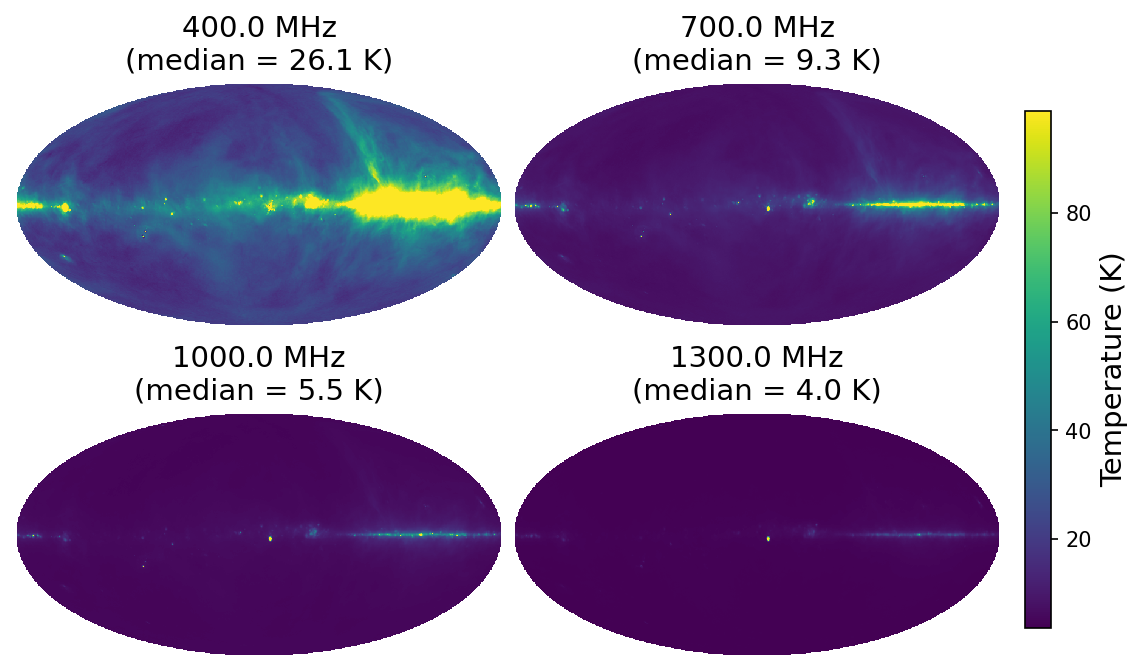
\includegraphics[width=1\linewidth]{../thesis/plots/sensitivity/background_only.png}
      \par\medskip
      {\footnotesize Radio Background obtained from the 2016 Global Sky Model \citep{zhengImprovedModelDiffuse2017}.}
    \end{column}
  \end{columns}
\end{frame}

\begin{frame}{Sensitivity Maps}{Total Sensitivity}
  \begin{columns}[T]
    \begin{column}{0.5\linewidth}
      \begin{itemize}
        % \item Total CHORD sensitivity including radio background
        \item Sensitivity is highly spatially and frequency dependent.
      \end{itemize}
    \end{column}
    \begin{column}{0.5\linewidth}
      \centering
      {\usebeamercolor[fg]{structure}Total CHORD Sensitivity}
      \par\smallskip
      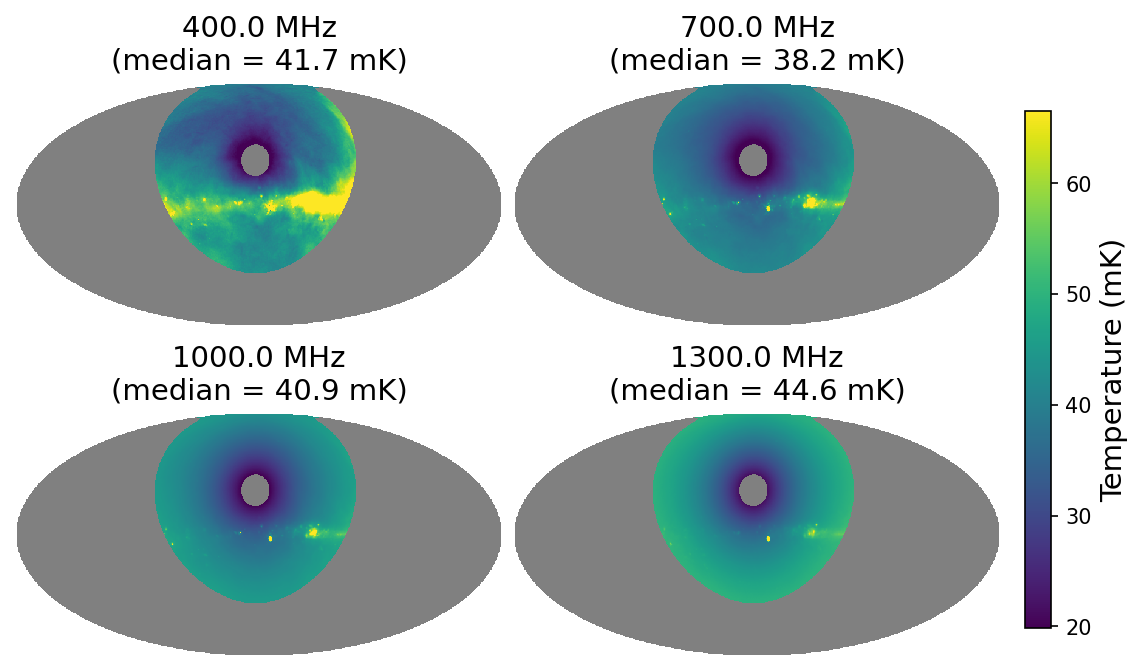
\includegraphics[width=1\linewidth]{../thesis/plots/sensitivity/total_noise.png}
      \par\medskip
      {\footnotesize Total CHORD brightness temperature sensitivity over the CHORD observing range.}
    \end{column}
  \end{columns}
\end{frame}

\subsection{Impact of RRL stacking and smoothing}
\begin{frame}{Signal to Noise Ratio of RRLs}{Selected Regions}
  \begin{columns}[T]
    \begin{column}{0.5\linewidth}
      % \begin{itemize}
      %   \item RRLs' signal is stronger at low frequencies.\\
      %   \item Sensitivity (aka noise) changes depending on frequency and location.\\
      % \end{itemize}
      \par\medskip
      What is the signal-to-noise ratio (SNR) of RRL detections in different regions of the sky?\\
    \end{column}
    \begin{column}{0.5\linewidth}
      \centering
      {\usebeamercolor[fg]{structure}Map of regions for further analysis}
      \par\smallskip
      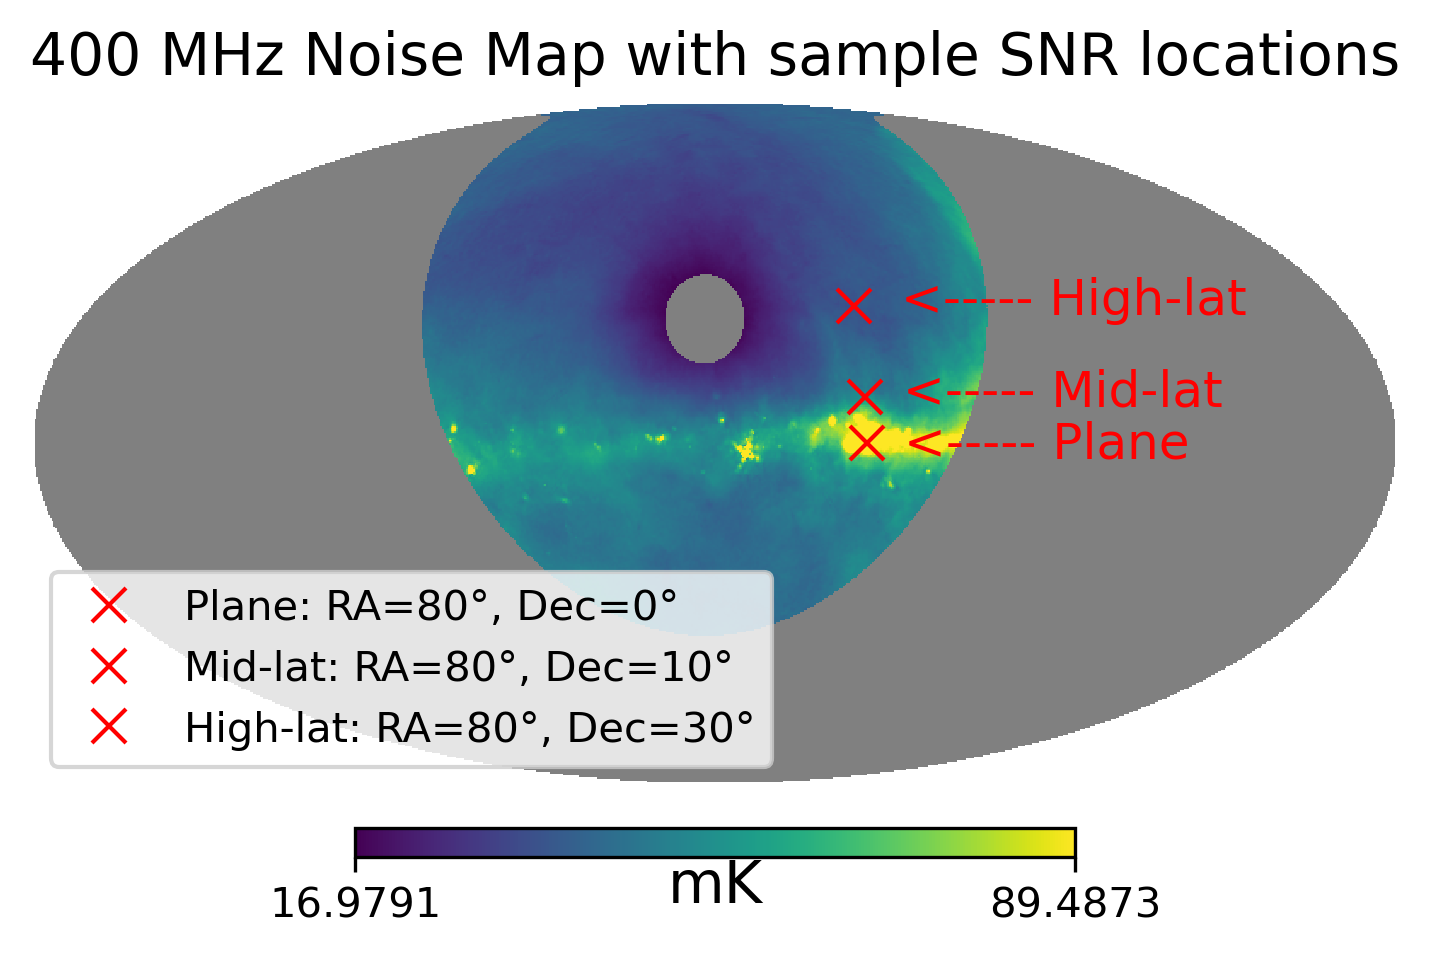
\includegraphics[width=0.8\linewidth, clip,trim=0 0 0 25pt]{../thesis/plots/sensitivity/snr_locations.png}
      \par\medskip
      {\footnotesize We take the median sensitivity over each region, Galactic plane, mid-latitude, and high-latitude.}
    \end{column}
  \end{columns}
\end{frame}

\begin{frame}{Signal to Noise Ratio of RRLs}{Native SNR per RRL}
  \begin{columns}[T]
    \begin{column}{0.5\linewidth}
      \centering
      {\usebeamercolor[fg]{structure}Native resolution}
      \par\smallskip
      \begin{tabular}{@{}lcc@{}}
        \toprule
        & \textbf{300 MHz} & \textbf{1.5 GHz} \\
        \midrule
        Angular Res. & $21'$              & $4.2'$ \\
        Velocity Res. & $5\ \mathrm{km\,s^{-1}}$ & $1\ \mathrm{km\,s^{-1}}$ \\
        \bottomrule
      \end{tabular}
      \par\medskip
      \begin{itemize}
        \item Low frequency has worse angular and velocity resolution.
        \item Low frequency has better SNR per line.
      \end{itemize}
    \end{column}
    \begin{column}{0.5\linewidth}
      \centering
      {\usebeamercolor[fg]{structure}SNR by region, using native resolutions}
      \par\smallskip
      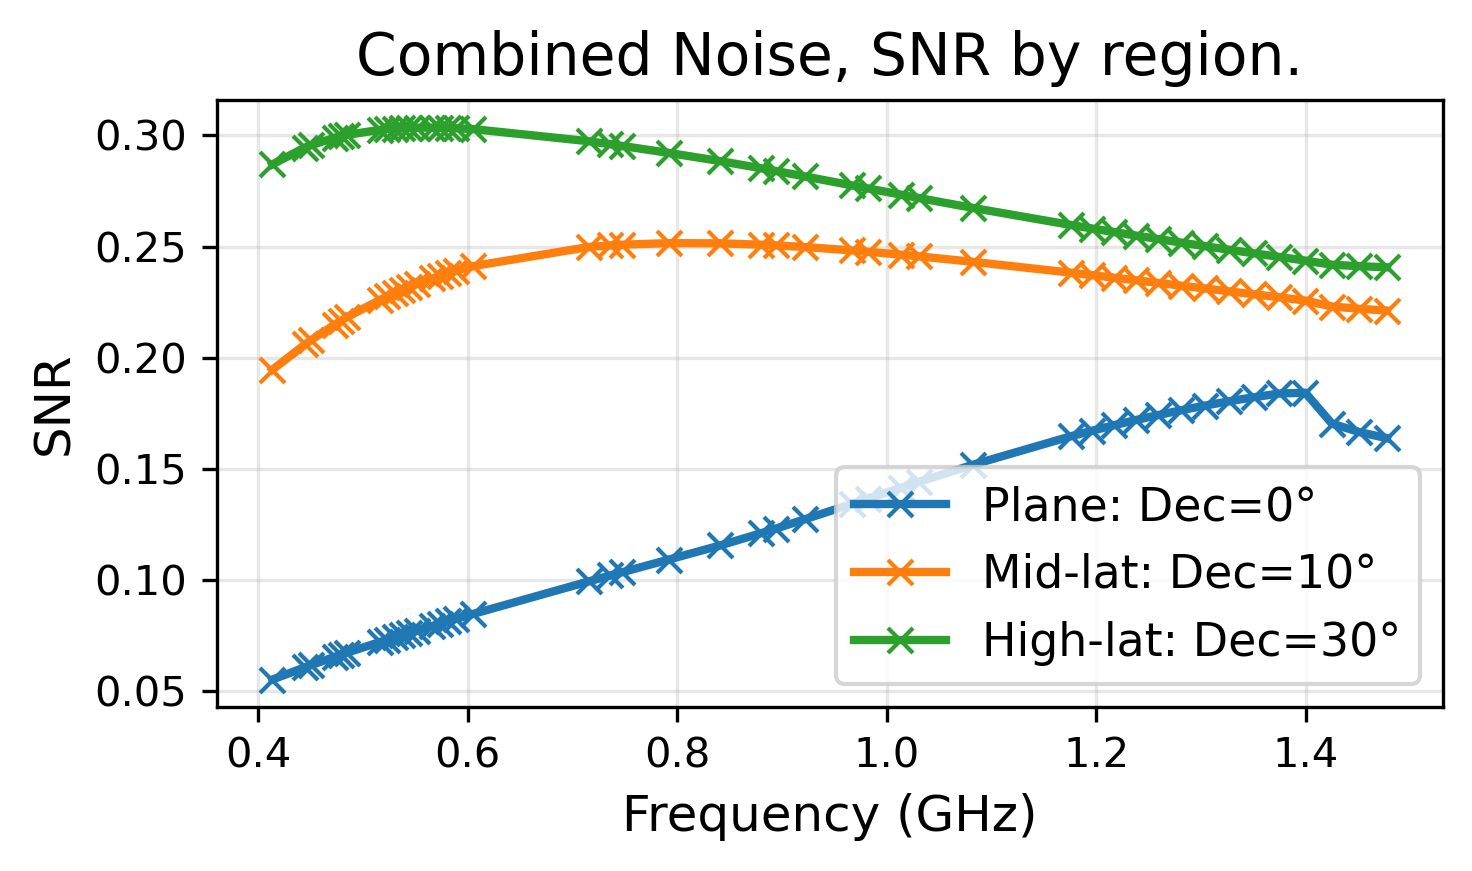
\includegraphics[width=1\linewidth, clip,trim=0 0 0 23pt]{../thesis/plots/sensitivity/snr_by_region.png}
      \par\medskip
      {\footnotesize Native SNR per RRL for each region, assuming a line intensity of 10 mK at 1.5 GHz.}
    \end{column}
  \end{columns}
\end{frame}

\begin{frame}{Signal to Noise Ratio of RRLs}{SNR with smoothing}
  \begin{columns}[T]
    \begin{column}{0.5\linewidth}
      \begin{itemize}
        \item Each line is smoothed to a 5 km s$^{-1}$ velocity resolution.
        \item Each line is smoothed to 22 arcminute angular resolution.\\
        \[
        N = \frac{\Omega_{\mathrm{smoothed}}}{\Omega_{\mathrm{native}}}
        \]
        \[
        \sigma_T [\text{smoothed}] = \frac{\sigma_T [\text{native}]}{\sqrt{N}}
        \]
        Where $N$ is the independent samples in the smoothed beam and $\sigma_T$ is the sensitivity.
      \end{itemize}
    \end{column}
    \begin{column}{0.5\linewidth}
      \centering
      {\usebeamercolor[fg]{structure}SNR by region, after smoothing}
      \par\smallskip
      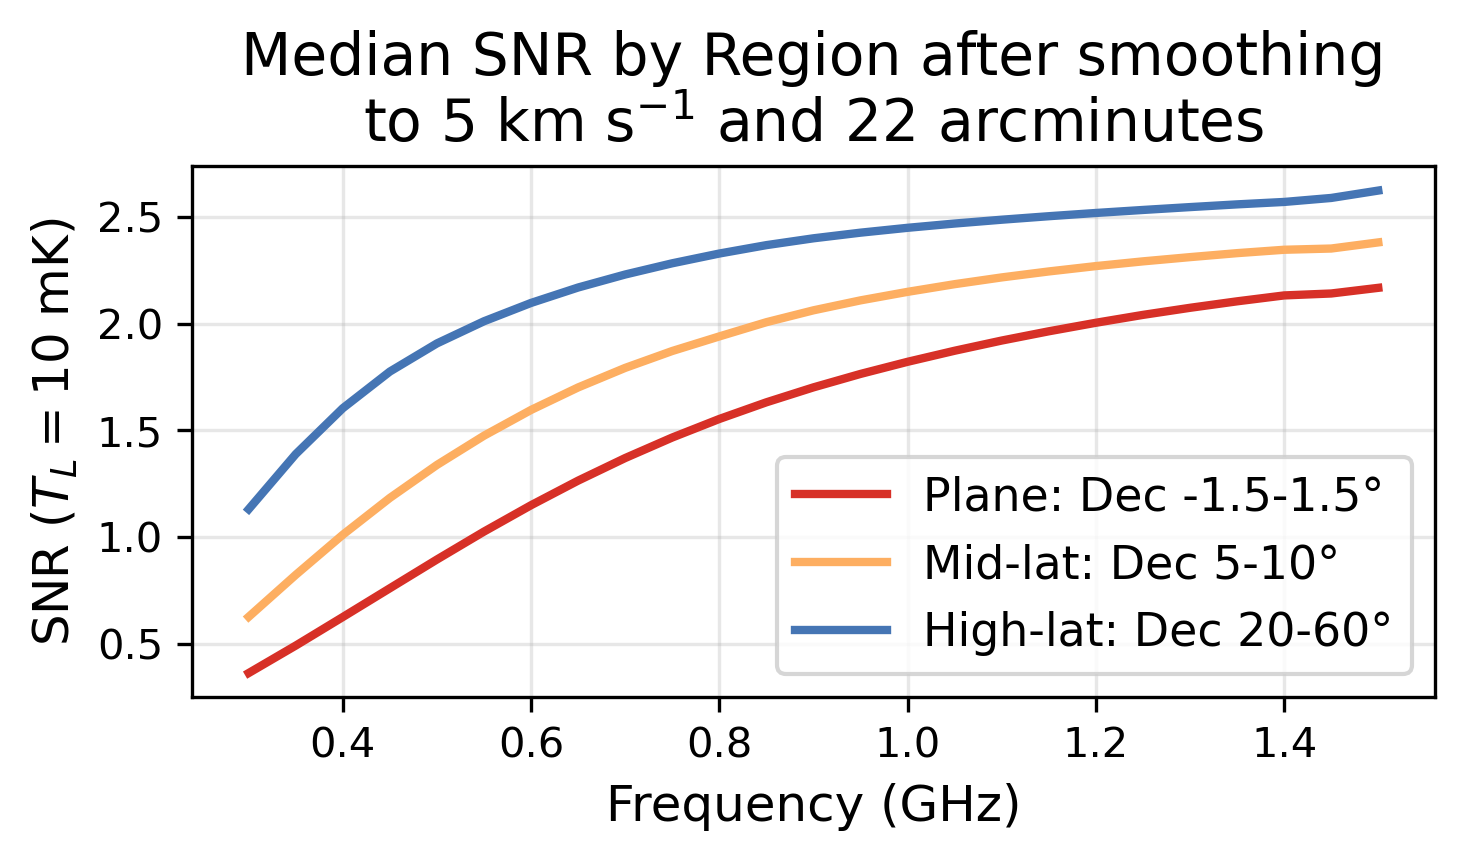
\includegraphics[width=1\linewidth, clip,trim=40pt 0 70pt 23.5pt]{../thesis/plots/sensitivity/smoothed_snr_by_region.png}
      \par\medskip
      {\footnotesize Smoothed SNR shows that high frequency RRLs now have the best SNR per line.}
    \end{column}
  \end{columns}
\end{frame}

\subsection{CHORD sensitivity compared to published SIGGMA survey}
\begin{frame}{CHORD detection of SIGGMA Results}{SIGGMA range}
  The Survey of Ionized Gas in the Galaxy Made with the Arecibo telescope (SIGGMA) made 427 RRL detections. 26 are within the CHORD survey area.\\
  \par\medskip
  \par\medskip
    \centering
    {\usebeamercolor[fg]{structure}RRL detections plotted on CHORD sensitivity map}
    \par\smallskip
    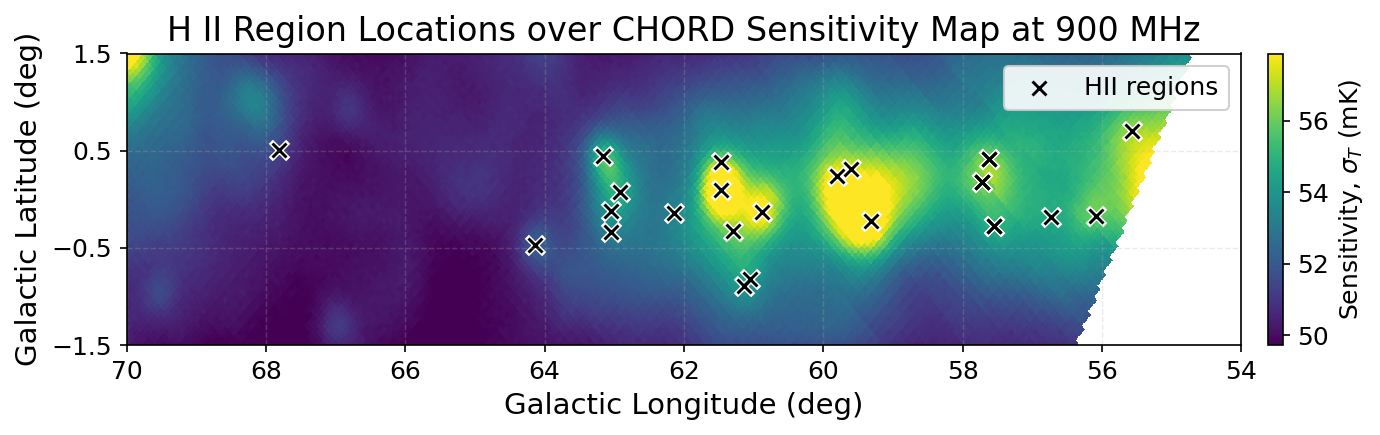
\includegraphics[width=0.7\linewidth, clip, trim=0 0 0 23pt]{../thesis/plots/siggma/hii_regions_over_chord_sensitivity.png}
    \par\medskip
    {\footnotesize The CHORD sensitivity at 900 MHz overlaid by the SIGGMA detections.}
\end{frame}

\begin{frame}{CHORD detection of SIGGMA Results}{SNR per smoothing level}
  \begin{columns}[T]
    \begin{column}{0.5\linewidth}
      \begin{itemize}
        \item I used the SIGGMA results to estimate expected Signal.
        \item I used CHORD sensitivity maps to estimate expected Noise.
        \item I smoothed to a common angular and velocity resolution.
      \end{itemize}
      \par\medskip
      The number of lines to stack depends on the angular smoothing level.\\
    \end{column}
    \begin{column}{0.5\linewidth}
      \centering
      {\usebeamercolor[fg]{structure}SNR of SIGGMA detections after smoothing}
      \par\smallskip
      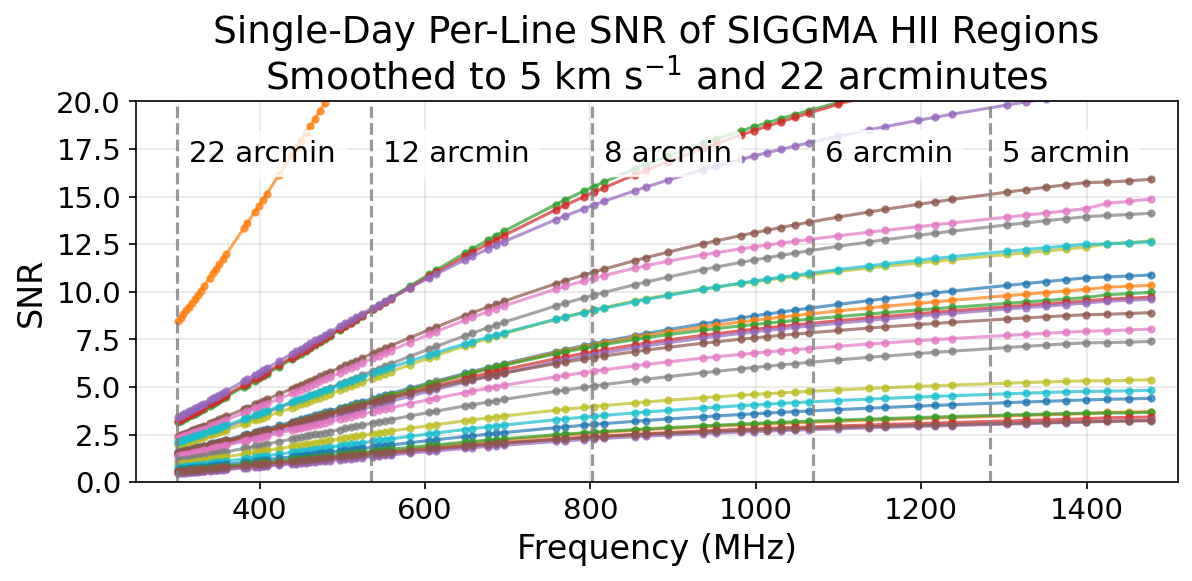
\includegraphics[width=1\linewidth, clip, trim=0 0 0 44pt]{../thesis/plots/siggma/SNR_per_SIGGMA_line_smoothed.png}
      \par\medskip
      {\footnotesize SNR smoothed to a common 22 arcminute resolution.}
    \end{column}
  \end{columns}
\end{frame}

\begin{frame}{CHORD detection of SIGGMA Results}{Detection Results}
  \centering
  {\usebeamercolor[fg]{structure}Stacked SNR per RRL detection with one observing day}
  \par\medskip
  \begin{tabular}{l c c c c}
    \toprule
    Order & Name & SNR $5'$ & SNR $6'$ & SNR $8'$ \\
    \midrule
    1 & G063.164+00.449 & $85.04 \pm 4.97$ & $130.52 \pm 7.63$ & $222.38 \pm 13.00$ \\
    2 & G061.473+00.094 & $41.86 \pm 3.23$ & $63.49 \pm 4.90$ & $105.47 \pm 8.14$ \\
    $\vdots$ & $\vdots$ & $\vdots$ & $\vdots$ & $\vdots$ \\
    25 & G062.142-00.144 & $2.03 \pm 0.31$ & $3.13 \pm 0.49$ & $5.42 \pm 0.84$ \\
    26 & G057.715+00.173 & $2.02 \pm 0.20$ & $3.11 \pm 0.31$ & $5.32 \pm 0.53$ \\
    \bottomrule
  \end{tabular}
  \par\medskip
  {\footnotesize Smoothing to $5'$, $6'$, $8'$ stacks 8, 14, and 27 lines respectively.}
  \par\medskip
  \par\medskip
  Conclusion: CHORD can detect all SIGGMA results within a single observing day.
\end{frame}

\begin{frame}{Sensitivity Analysis Limitations}
  \begin{itemize}
    \item The radio background used for $T_{sky}$ is limited to 56 arcminute resolution.
    \par\medskip
    \item We assumed the smoothed beam is an average over independent native beams, but true native beams have some spatial noise correlations.
    \par\medskip
    \item Frequency resolution is dependent on the upsampling hardware and might have limitations.
  \end{itemize}
\end{frame}

\section{Extension CHORD}
\subsection{How would adding more dishes improve CHORD's angular resolution?}
\begin{frame}{Why add more dishes?}
  Longer baselines provide smaller angular resolution.
  \centering
  \par\medskip
  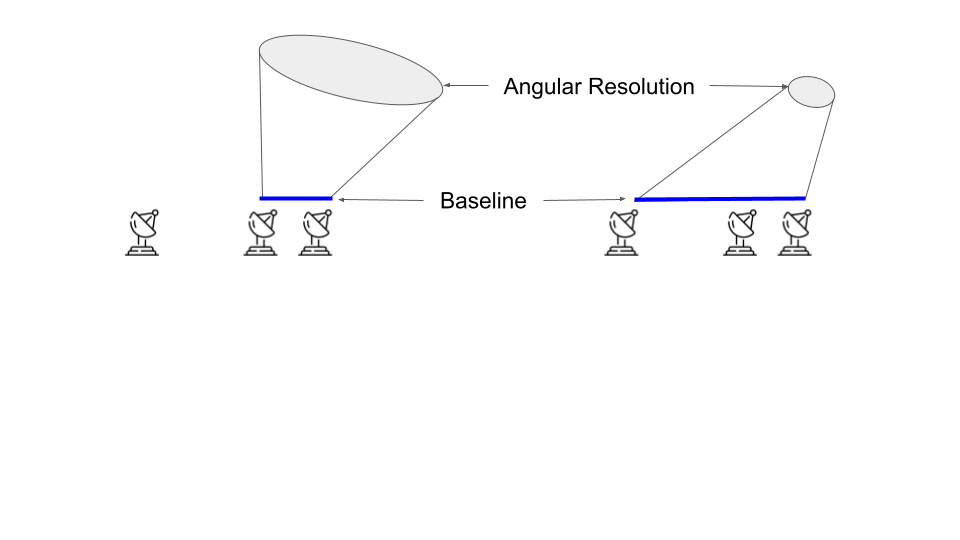
\includegraphics[width=0.9\linewidth,clip,trim=0 280pt 0 0]{plots/angular_resolution_diagram.png}
  \par\medskip
  \par\medskip
  \begin{itemize}
    \item Would more dishes improve angular resolution to RRLs?
    \item What is the optimal dish placement?
  \end{itemize}
\end{frame}

\begin{frame}{Candidate locations}
  \centering
  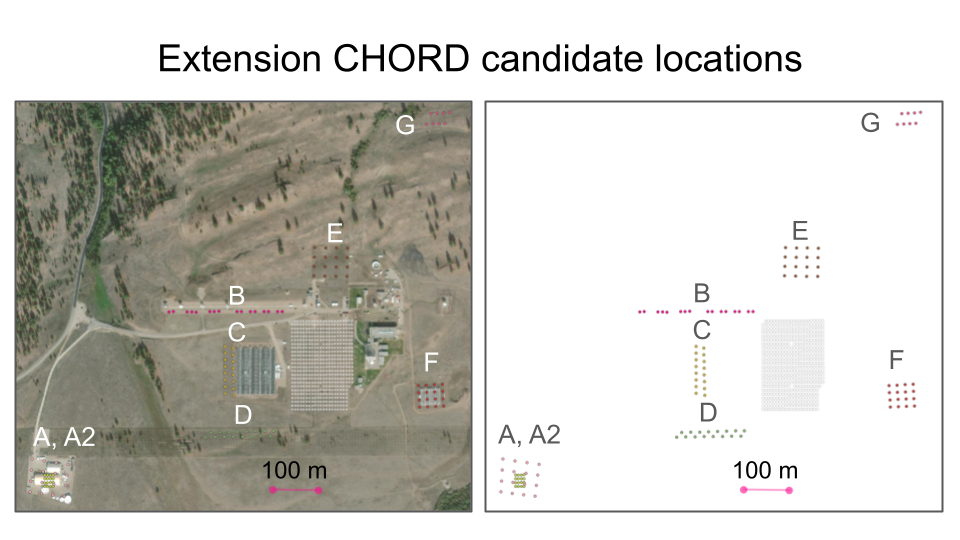
\includegraphics[width=0.8\linewidth,clip,trim=0 0 0 0]{../thesis/plots/ext_chord/site_map_v2.png}
\end{frame}

\begin{frame}{Location A, the longest possible baseline}
  \centering
  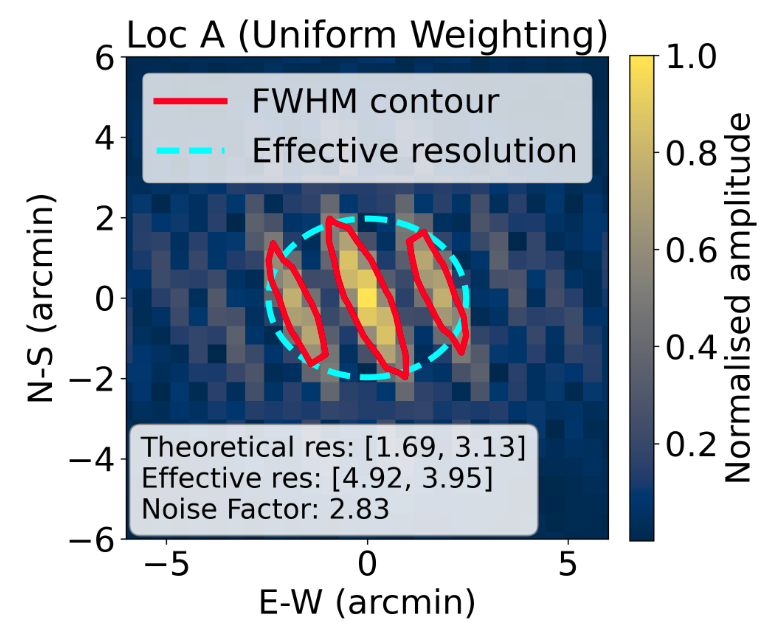
\includegraphics[width=0.5\linewidth,clip,trim=0 0 0 0]{plots/Location_A.png}
  \par\medskip
  Despite having the longest baseline, Location A is not the best option.
\end{frame}

\begin{frame}{Location B + D, the best overall combination}
  \centering
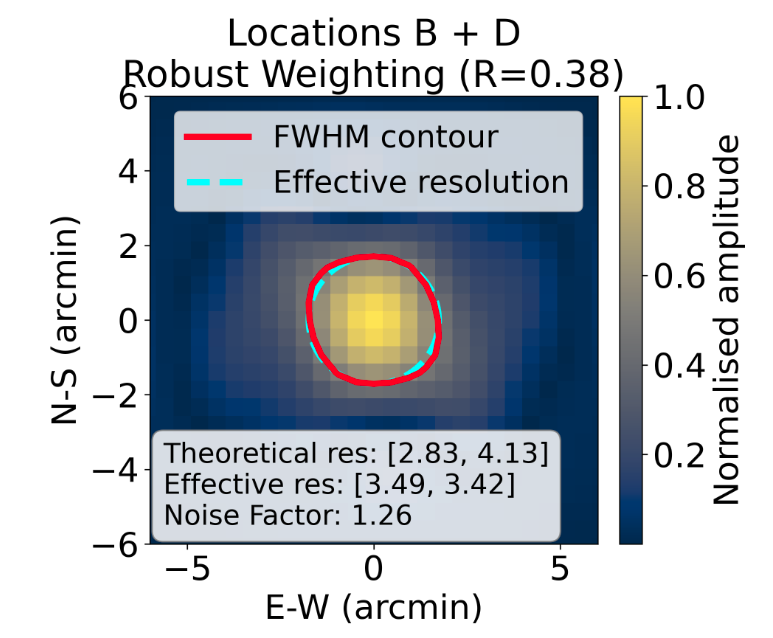
\includegraphics[width=0.5\linewidth,clip,trim=0 0 0 0]{plots/Locations_B_D.png}
\par\medskip
Angular resolution decreased by 44\% while noise increased by 26\%.
\end{frame}
\section*{Conclusions}
\begin{frame}{Conclusions}
  \begin{columns}[T]
    \begin{column}{0.55\linewidth}
    Can CHORD detect RRLs?
    \begin{itemize}
      \item I created an RFI detection pipeline and found 79 of the 116 Hn$\alpha$ RRLs are RFI-free.
      \item I showed CHORD can reproduce all SIGGMA detections.
    \end{itemize}
    \par\smallskip
    What sensitivity can be achieved?
    \begin{itemize}
      \item I provide sensitivity maps and stacked SNR methods given a desired smoothing.
    \end{itemize}
    \par\smallskip
    What angular resolution can be achieved?
    \begin{itemize}
      \item Extension-CHORD could yield 44\% improvement for a 26\% noise cost.
    \end{itemize}
    \end{column}
    \begin{column}{0.45\linewidth}
      \centering
      {\usebeamercolor[fg]{structure}RFI Classifications}
      \par\smallskip
      \includegraphics[width=1\linewidth, clip,trim=0 0 0 33pt]{../thesis/plots/rfi/RFI_flagged_spectrum.png}
      \par\medskip
      {\usebeamercolor[fg]{structure}Total Sensitivity}
      \par\smallskip
      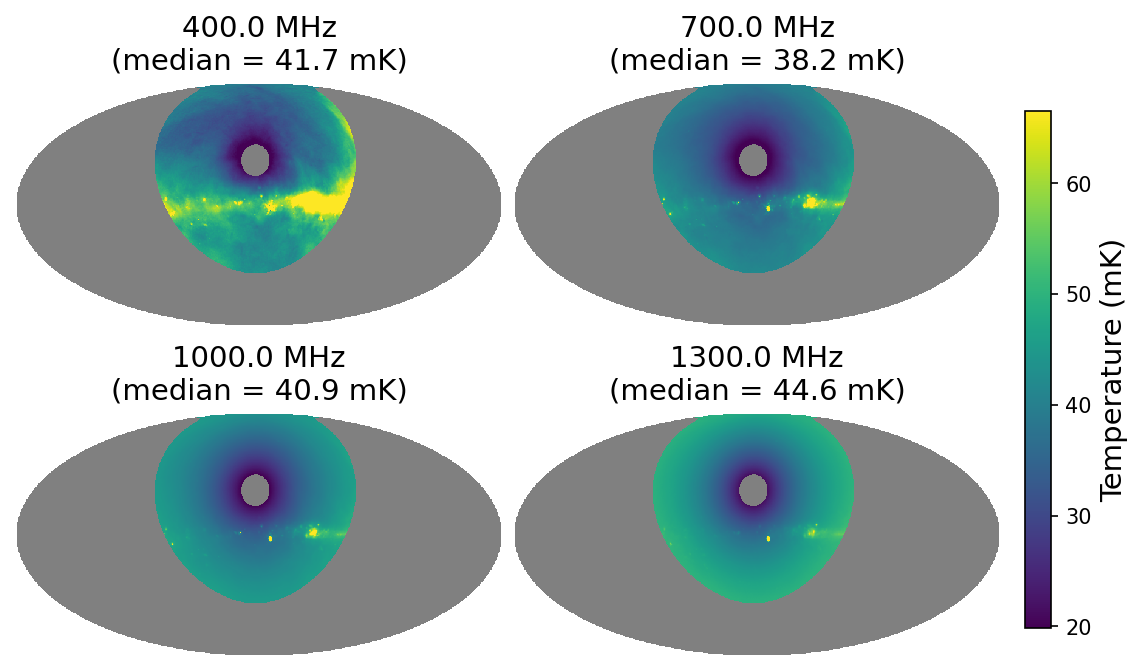
\includegraphics[width=1\linewidth, clip,trim=0 158pt 60pt 0]{../thesis/plots/sensitivity/total_noise.png}

    \end{column}
  \end{columns}
\end{frame}

% Exclude the references (and anything after) from the page count and hide the
% footer number on them. \appendix caps the X/Y total at the last content slide;
% redefining Cookie's \cookie@numbering to none blanks the footer number for all
% following frames (the theme reads this macro per-frame at shipout); and
% noframenumbering stops the references frame from advancing the counter.
\appendix
\makeatletter\def\cookie@numbering{none}\makeatother

% \section*{References}
\begin{frame}[allowframebreaks,noframenumbering]{References}
  \footnotesize
  \bibliographystyle{apj}
  \bibliography{references}
\end{frame}

% Backup slides: number them on their own, restarting from 1. Switch Cookie to
% plain counter mode (number only, no fraction) and reset the frame counter.
% Cookie derives the X/Y total from the frame counter's value at end of
% document, so we first save the content total and restore it before
% \end{document} (see below) — otherwise the reset here would make the main
% slides read X/12 instead of X/28.
\newcounter{cookiemaintotal}
\setcounter{cookiemaintotal}{\value{framenumber}}
% \makeatletter\def\cookie@numbering{counter}\makeatother
% \setcounter{framenumber}{0}
\section{Appendix}
\begin{frame}{RFI Detection}{Spectral Kurtosis definition}
  \begin{columns}[T]
    \begin{column}{0.5\linewidth}
      \begin{itemize}
        \item System noise and astronomical signals are Gaussian distributed over time, while RFI is not.
        \item Spectral Kurtosis (SK) \citep{nitaGeneralizedSpectralKurtosis2010} is a measure of Gaussianity in a power timeseries.
        \item For a Gaussian voltage timeseries, the spectral kurtosis is 1.
      \end{itemize}
    \end{column}
    \begin{column}{0.5\linewidth}
      \centering
      {\usebeamercolor[fg]{structure}The generalized spectral kurtosis estimator:}
      \begin{align*}
          \text{let:} \quad S_1 &= \sum_{j=1}^{M} P_{N,j}, \quad S_2 = \sum_{j=1}^{M} P_{N,j}^2 \\[4pt]
          \widehat{SK} &= \frac{M N d + 1}{M - 1} \left( \frac{M S_2}{S_1^2} - 1 \right),
      \end{align*}
      {\footnotesize Where $P_{N}$ is the integrated power per frequency channel, $M$ is the number of integrated time samples, $Nd$ is the number of independent time samples per integration.}
    \end{column}
  \end{columns}
\end{frame}

\begin{frame}{RFI Detection}{Spectral Kurtosis Calibration}
  \begin{columns}[T]
    \begin{column}{0.5\linewidth}
      \begin{itemize}
        \item We used RFI free data from the RFI protected band of 1400-1430 MHz to calibrate the SK estimator.
        \item This is required since the RFI monitor does not obtain perfectly independent time samples, which biases the estimator.
        \item The calibrated shape parameter is found to be $Nd = 2500\cdot 15/16 \times 0.96$
      \end{itemize}
    \end{column}
    \begin{column}{0.5\linewidth}
      \centering
      {\usebeamercolor[fg]{structure}SK calibration}
      \par\smallskip
      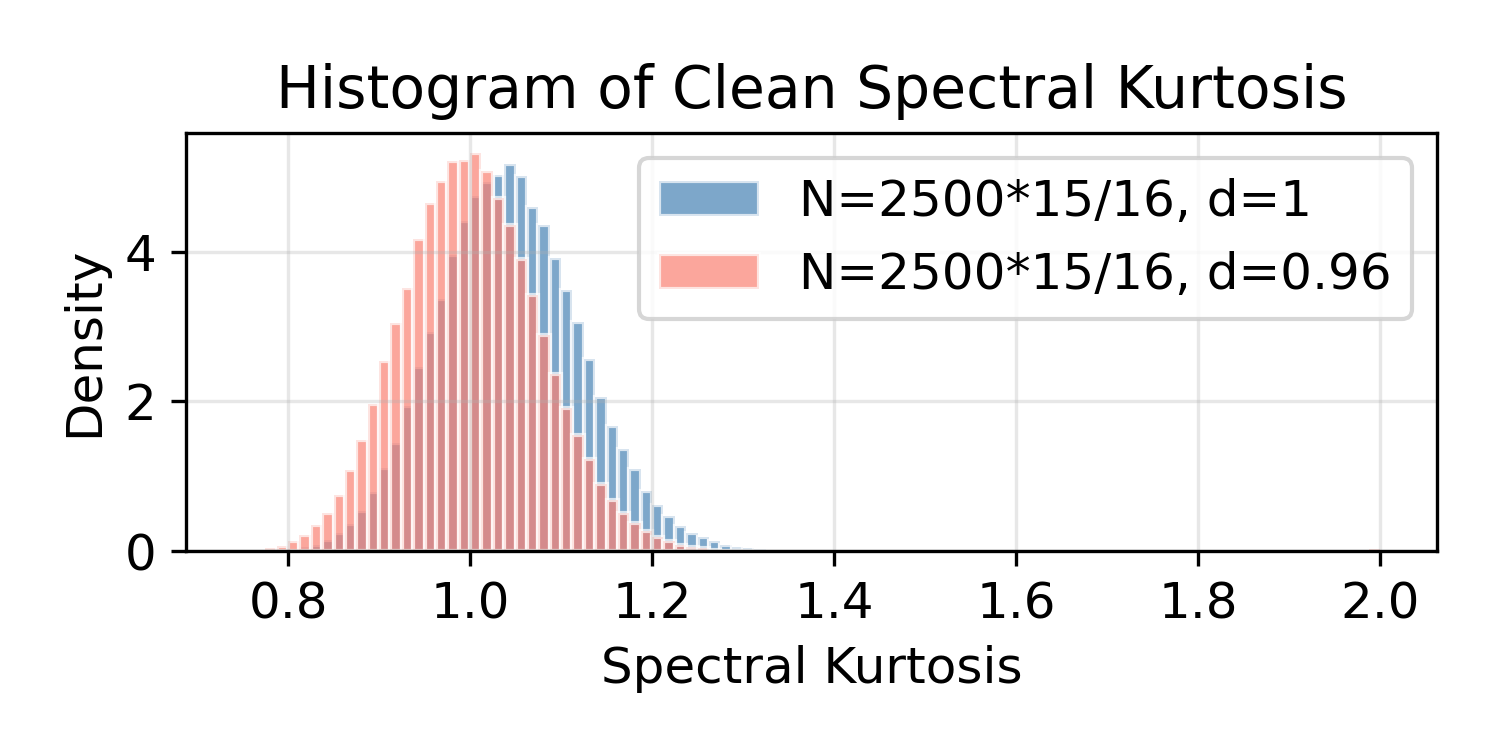
\includegraphics[width=1\linewidth]{../thesis/plots/rfi/hist_setting_sk_p.png}
      \par\medskip
      {\footnotesize The SK estimator (blue) is calibrated on clean data (red) to have a mode of exactly 1.}
    \end{column}
  \end{columns}
\end{frame}

\begin{frame}{RFI Detection}{Spectral Kurtosis RFI thresholds}
  \begin{columns}[T]
    \begin{column}{0.5\linewidth}
      \begin{itemize}
        \item The RFI-free SK distribution is simulated with $10^5$ Monte Carlo draws from $\texttt{Gamma}(Nd, 2\sigma^2)$.
        \item The observed SK in the clean 1400--1430 MHz band matches these simulations, confirming the band is RFI free.
        \item The simulated 0.1\% and 99.9\% quantiles set the detection thresholds: SK values outside them are flagged as RFI.
      \end{itemize}
    \end{column}
    \begin{column}{0.5\linewidth}
      \centering
      {\usebeamercolor[fg]{structure}Null SK distribution with RFI detection thresholds}
      \par\smallskip
      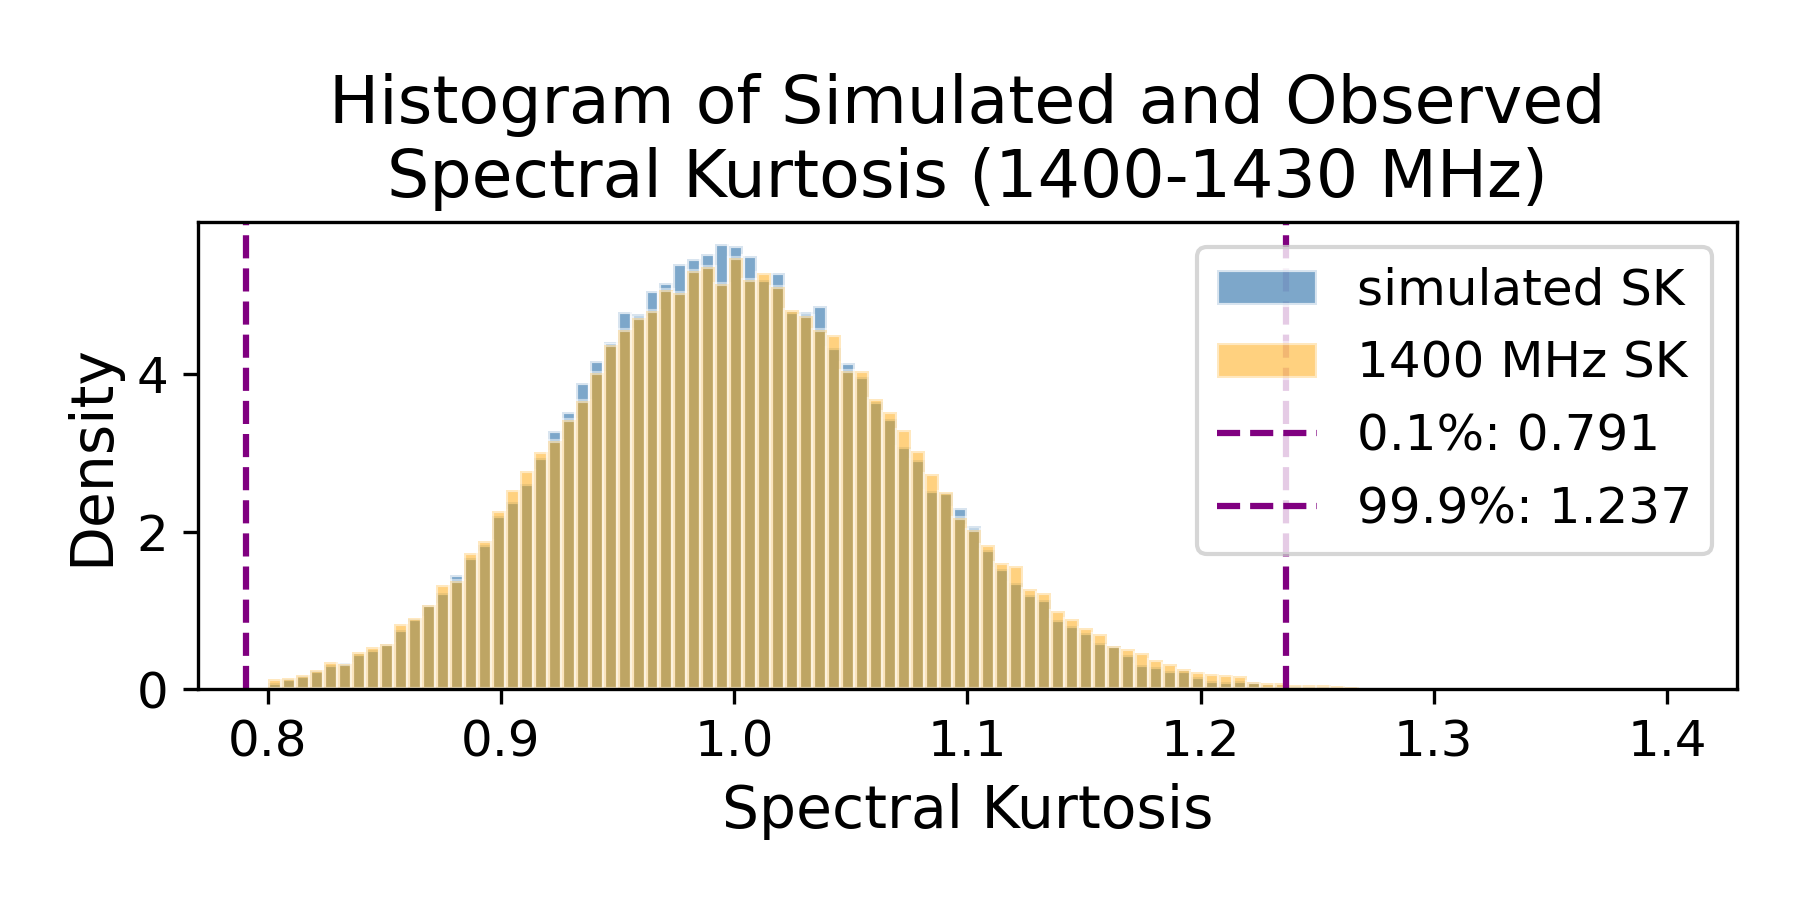
\includegraphics[width=1\linewidth]{../thesis/plots/rfi/spectral_kurtosis_all_time.png}
      \par\medskip
      {\footnotesize Simulated null SK distribution (blue) matches with observed non-RFI SK (red). RFI thresholds are taken as the 0.1\% and 99.9\% quantiles.}
    \end{column}
  \end{columns}
\end{frame}

\begin{frame}{RFI Detection}{SK flagging results}
  \begin{columns}[T]
    \begin{column}{0.5\linewidth}
      \centering
      {\usebeamercolor[fg]{structure}Power and SK on RFI spectrum}
      \par\smallskip
      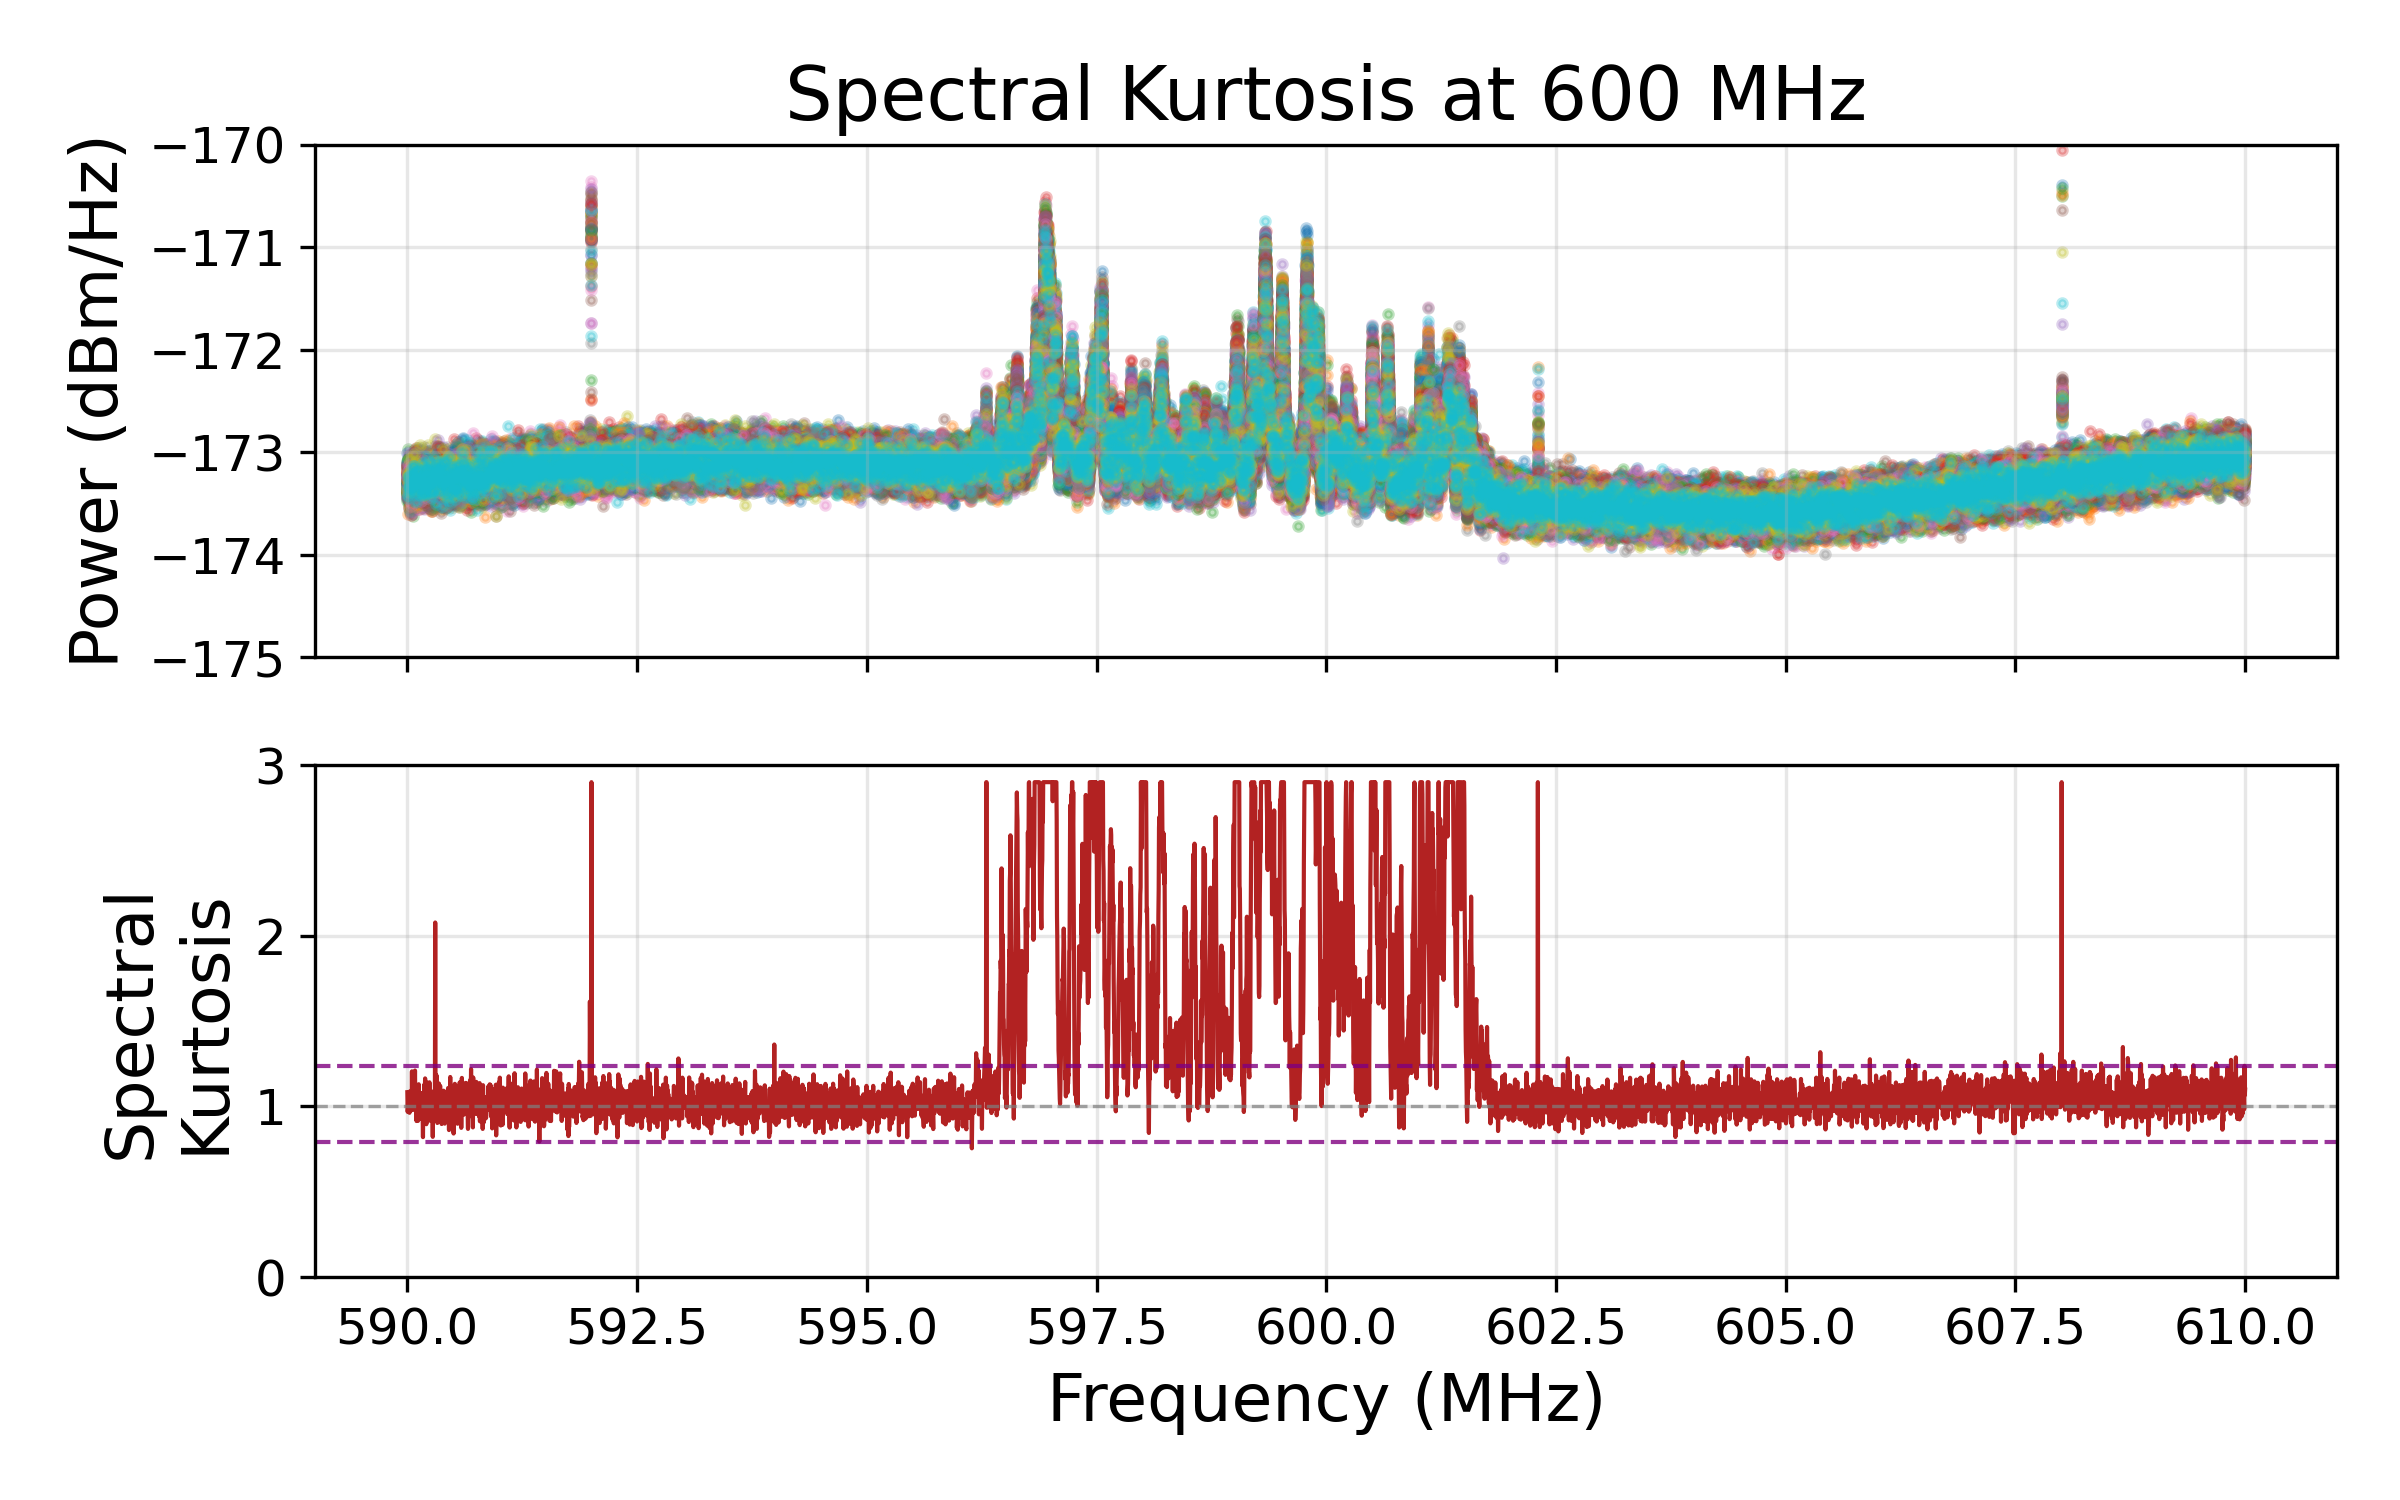
\includegraphics[width=1\linewidth]{../thesis/plots/rfi/600MHz_sample_SK.png}
      \par\medskip
      {\footnotesize SK (bottom) identifies RFI-affected Power spectrum (top).}
    \end{column}
    \begin{column}{0.5\linewidth}
      \centering
      {\usebeamercolor[fg]{structure}RFI flagging results, full CHORD band}
      \par\smallskip
      \includegraphics[width=1\linewidth]{../thesis/plots/rfi/RFI_flagged_spectrum.png}
      \par\medskip
      {\footnotesize RFI monitor power colored by SK RFI flagging results. In total 75.6\% of the CHORD band is found to be RFI free.}
    \end{column}
  \end{columns}
\end{frame}

\begin{frame}{Line Characterization}{Gaussian weighted average around each RRL}
  \begin{columns}[T]
    \begin{column}{0.5\linewidth}
      \begin{itemize}
        \item For a line to be detectable, it should be mostly RFI free within $\pm 200 \text{ km/s}$.
        \item We compute a per line score as a Gaussian weighted average of the binary RFI labels centered at the rest frequency with a standard deviation of $\sigma_f = 100 \text{ km/s}$
      \end{itemize}
      \begin{align*}
        s = \frac{\sum_i w_i\, \text{RFI}_i}{\sum_i w_i},~~w_i = \exp\!\left(-\frac{(f_i - f_0)^2}{2\sigma_f^2}\right)
      \end{align*}
    \end{column}
    \begin{column}{0.5\linewidth}
      \centering
      {\usebeamercolor[fg]{structure}Clean Scores}
      \par\smallskip
      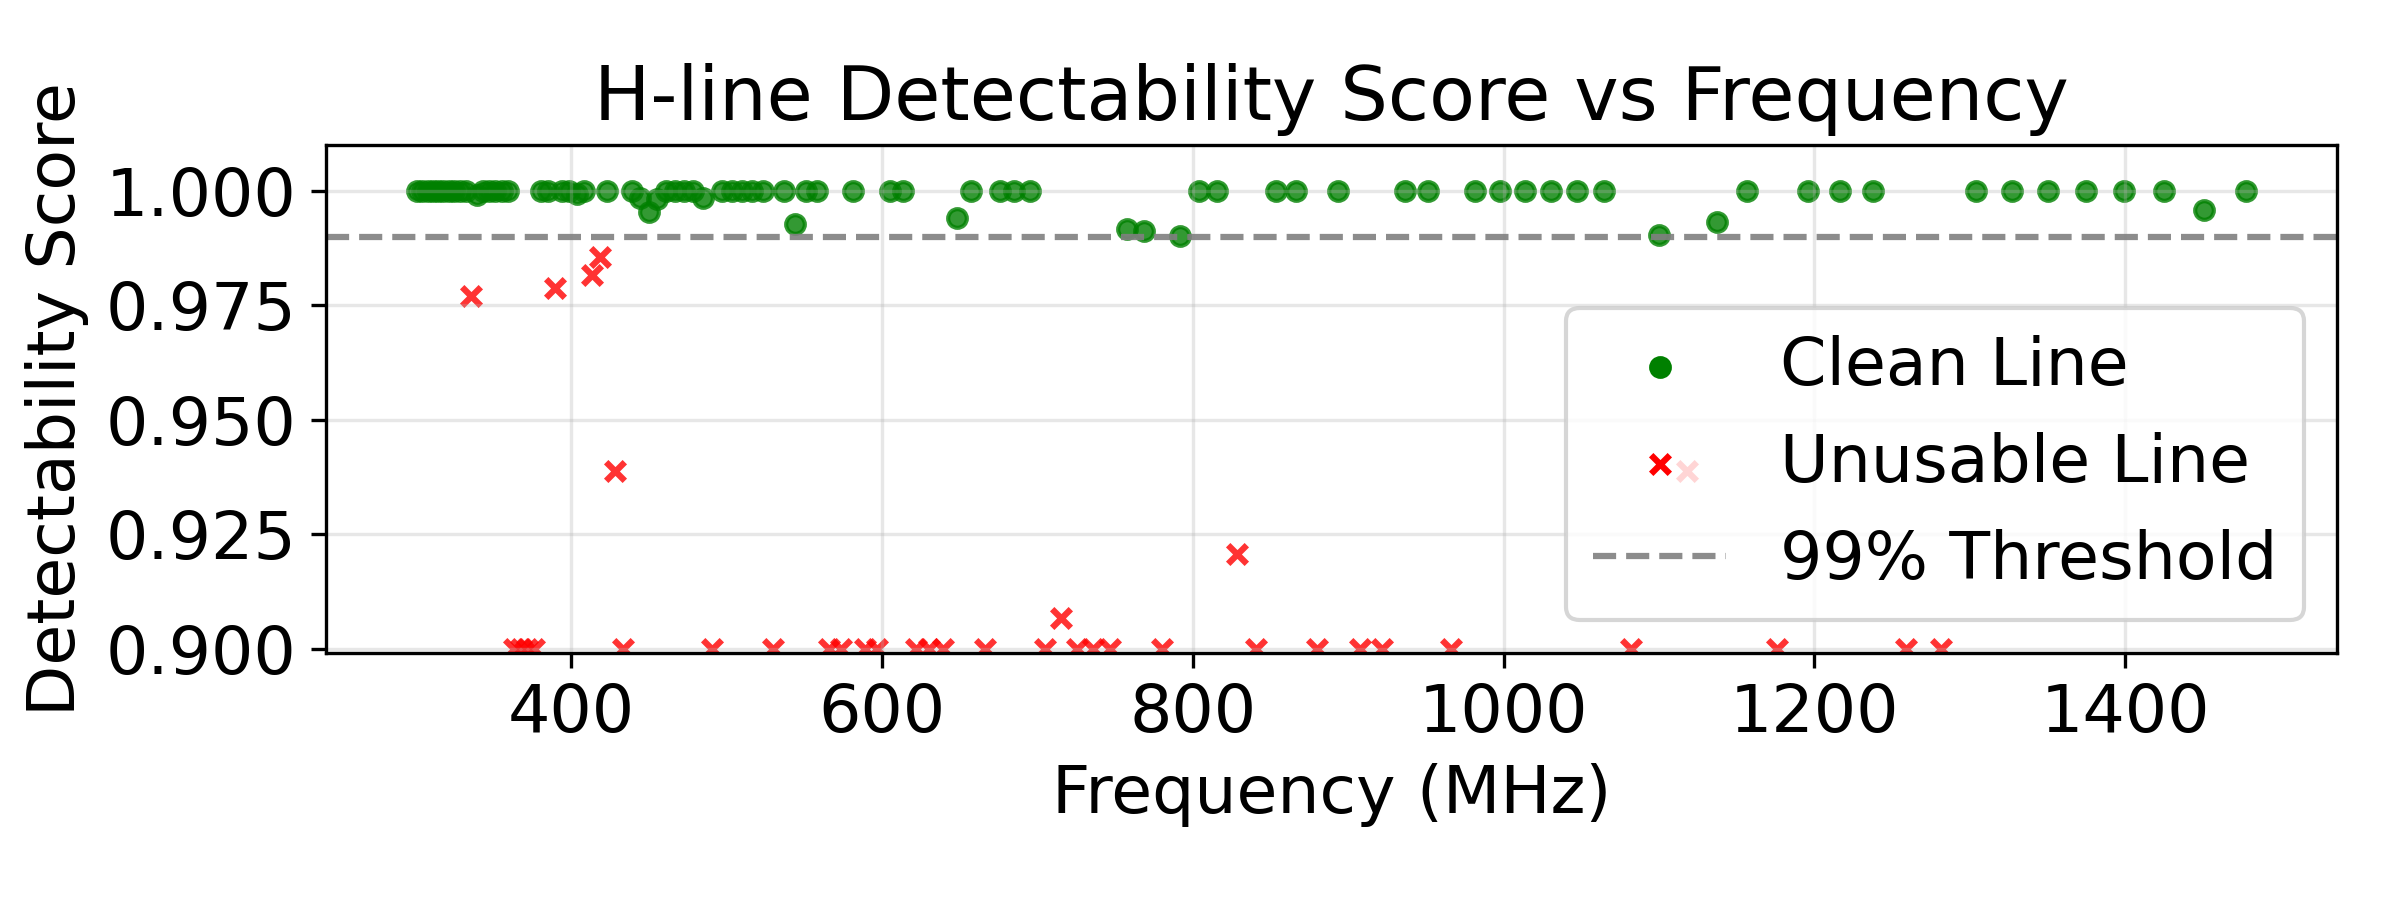
\includegraphics[width=1\linewidth]{../thesis/plots/rfi/h_line_clean_score.png}
      \par\medskip
      {\footnotesize Per line clean scores for all 116 Hn$\alpha$ RRLs in the CHORD band. Lines with a score $>0.99$ are considered detectable.}
    \end{column}
  \end{columns}
\end{frame}

\begin{frame}{Line Characterization}{Detectable Lines by Frequency Range}
  \centering
  {\usebeamercolor[fg]{structure}Detectable vs.\ RFI-contaminated Hn$\alpha$ RRLs}
  \par\medskip
  \begin{tabular}{lrr}
    \toprule
    \textbf{Frequency Range} & \textbf{Detectable} & \textbf{Contaminated} \\
    \textbf{(MHz)} & \textbf{Transitions} & \textbf{Transitions} \\
    \midrule
    300--470   & 29 & 10 \\
    470--800   & 23 & 16 \\
    800--1500  & 27 & 11 \\
    \midrule
    \textbf{Total} & \textbf{79} & \textbf{37} \\
    \bottomrule
  \end{tabular}
  \par\medskip
\end{frame}

\begin{frame}{Limitations}{}
\begin{itemize}
    \item CHORD is orders of magnitude more sensitive than the RFI monitor, signals that are not detectable by the RFI monitor may nonetheless impede CHORD.
    \item CHORD has a directional beam pointed upwards while the RFI monitor is most sensitive downwards and horizontally, RFI from overhead may be missed by the RFI monitor.
    \item This analysis is based on a single hour of RFI monitor data, which may not be representative of the long-term RFI environment.
    \item RFI changes over time, as new RFI sources emerge, spectrum currently free of RFI might become corrupted.
\end{itemize}
\end{frame}

\begin{frame}{Sensitivity Definitions}{Point Source Sensitivity}

  A telescope's sensitivity, choosing a signal-to-noise ratio (SNR) of 1, is equivalent to the root mean square (RMS) noise of the telescope.\\
  ~\\
  The point-source RMS noise follows the radiometer equation, which for dual polarization is given by
  \[
  \sigma_{\mathrm{RMS}}\,[\mathrm{Jy/beam}] = \frac{2k\,(T_{\mathrm{ant}}+T_{\mathrm{sky}})}{A_e\sqrt{2\,\Delta\nu\,\tau_{\mathrm{eff}}\,N(N-1)}}
  \]
  where $k$ is Boltzmann's constant, $T_{\mathrm{ant}}$ is the antenna temperature, $T_{\mathrm{sky}}$ is the sky temperature, $A_e$ is the effective area of a single dish, $\Delta\nu$ is the bandwidth, $\tau_{\mathrm{eff}}$ is the effective integration time, and $N$ is the number of dishes.
\end{frame}

\begin{frame}{Sensitivity Definitions}{Angular Resolution}
  The angular resolution is the smallest angular scale the telescope can resolve. It is defined as the full width at half maximum (FWHM) of the synthesized beam, which is the combined beam after correlating all pairs of dishes in the interferometer.\\
  ~\\
  The angular resolution of an interferometer is set by the longest baseline between two dishes ($D_{\mathrm{EW}}$ and $D_{\mathrm{NS}}$) and the observing wavelength ($\lambda$),
  \[
  \theta_{\mathrm{FWHM}} = \frac{\lambda}{D_{\mathrm{EW}}}, \quad \phi_{\mathrm{FWHM}} = \frac{\lambda}{D_{\mathrm{NS}}}.
  \]
  The beam solid angle is the area subtended by the synthesized beam,
  \[
  \Omega_s = \frac{\pi}{4\ln 2}\,\theta_{\mathrm{FWHM}}\,\phi_{\mathrm{FWHM}}.
  \]
\end{frame}


\begin{frame}{Sensitivity Definitions}{Brightness Temperature Sensitivity}

  Brightness temperature sensitivity, is a measure of the telescope's ability to detect extended sources. It is obtained by dividing the point-source RMS noise by the beam solid angle, and converting from Jy/beam to K by applying the Rayleigh-Jeans limit.\\
  ~\\
  \[
  \sigma_T\,[\mathrm{K}] = \frac{\sigma_{\mathrm{RMS}}}{\Omega_s}\,
\frac{c^2}{2k\nu^2}
  \]
\end{frame}

\begin{frame}{Line Strength}{}
  Emission intensity of an RRL is a function of the physical quantities of the ISM and the transition frequency. Peak line strength is given by \citet{andersonGBTDiffuseIonized2021} as
  \begin{equation*}
    \left( \frac{T_L}{\text{K}} \right) \backsimeq 3076~\left(\frac{T_e}{\text{K}}\right)^{-3/2}\left(\frac{EM}{\text{pc cm}^{-6}}\right) \left(\frac{\nu_0}{\text{GHz}}\right)^{-1} \left(\frac{\Delta V}{\text{km s}^{-1}} \right)^{-1} \Delta n M_{\Delta n},
    \label{eq:line_intensity}
  \end{equation*}

where:
\begin{itemize} 
  \item $T_e$, the electron temperature, $EM$, the emission measure, and $\Delta V$, the line width, are physical quantities of the ISM. 
  \item $\Delta n M_{\Delta n}$ is a quantum mechanical factor that is constant for all $n\alpha$ transitions. 
  \item $\nu_0$ is the rest frequency of the transition. \\
  \item \textbf{Meaning Line strength increases at lower frequencies.}
\end{itemize}
\end{frame}

\begin{frame}{Stacking}{}
  \begin{columns}[T]
    \begin{column}{0.5\linewidth}
      \begin{itemize}
        \item RRLs of different frequencies are all produced by the same underlying physical quantities; gas temperature and density.
        \item Measurement uncertainty is reduced by averaging signal from multiple RRLs.
        \item Inverse-variance weighting is used to combine signals having different SNR levels.
      \end{itemize}
    \end{column}
    \begin{column}{0.5\linewidth}
      \centering
      {\usebeamercolor[fg]{structure}Inverse-variance weighted average:}
      \par\smallskip
      \begin{equation*}
        \hat{\mu} = \frac{\sum_i^N x_i w_i }{\sum_i^N w_i}, \quad \text{Var}(\hat{\mu}) = \frac{1}{\sum_i^N w_i},
      \end{equation*}
      \begin{equation*}
        w_i = \frac{1}{\sigma_i^2},
      \end{equation*}
      \begin{equation*}
        \text{SNR} = \frac{\hat{\mu}}{\sqrt{\text{Var}(\hat{\mu})}} = \frac{\sum_i^N x_i w_i}{\sqrt{\sum_i^N w_i}}.
      \end{equation*}
      \par\medskip
      {\footnotesize Combined signal ($\hat{\mu}$), uncertainty ($\text{Var}(\hat{\mu})$) and SNR after stacking $N$ lines.}
    \end{column}
  \end{columns}
\end{frame}

% Restore the frame counter to the content total so the X/Y on the main slides
% reads the number of content slides, not the backup count.
\setcounter{framenumber}{\value{cookiemaintotal}}

\end{document}